\chapter{大型切伦科夫中微子望远镜}
\label{ch:neutrino_telescope}

来自宇宙中的中微子的流量比较微弱,Waxman和Bahcall假设产生高能宇宙线的源对于$\pi$介子产生过程并非是不透明的,即并没有隐藏的超高能宇宙线源。由此他们根据观测到的超高能宇宙线的流量,利用章节\ref{subsubsec:neutrino_production}中所讨论的宇宙线产生中微子的方式,推导得到了著名的Waxman-Bahcall上限\cite{Waxman_Bahcall_bound:1999, Waxman_Bahcall_bound:2001}:
\begin{equation}
    E_\nu^2 \Phi_\nu < E_\nu^2 \Phi_\nu^{\mathrm{WB}} = 5 \times 10^{-8} \mathrm{GeV} \mathrm{cm}^{-2} \mathrm{~s}^{-1} \mathrm{sr}^{-1} ,
    \label{eq:Waxman_Bahcall_bound}
\end{equation}
其中$E_\nu$表示高能中微子的流量,$\Phi_\nu$表示中微子的流量,$\Phi_\nu^{\mathrm{WB}}$表示满足假设的情况下最大的中微子流量。
考虑到中微子与物质的作用几率非常的小,因此他们推断只有当靶物质的质量达到$10^{12}\,\mathrm{kg}$,$\mathrm{km}^3$量级,即体积达到$\mathrm{km}^3$量级之后,才有可能在年的时间制度内探测到宇宙中的高能中微子信号。

通过建造大体积的切伦科夫光中微子望远镜来探测高能天体中微子的想法早在1950年代便已经被提出了\cite{Telescope_history:2019}。
1960 年,M. Markov 发表了他的突破性想法 \cite{Markov:1960},即在湖泊或海洋等大型天然水体的深处安装光敏探测器阵列,从而实现对超大体积的介质进行监控。
这种望远镜借助了天然的介质来作为中微子反应的靶物质,是在人类在目前生产力水平下实现体积达到$10^{12}\,\mathrm{kg}$,$\mathrm{km}^3$级别的靶物质质量的有效途径。
而且它利用了粒子产生的切伦科夫光信号,这是因为介质中切伦科夫光信号的衰减距离($30-100\,\mathrm{m}$)要远远长于除缪子以外的大多数带电粒子($1,\mathrm{cm}-1\,\mathrm{m}$),从而可以扩大单个探测器的有效探测体积。
因此,望远镜中的光敏探测阵列可以布置得比较稀疏($~\mathcal{O}(100)\,\mathrm{m}$),从而实现以比较低廉的成本来监控如此庞大体积的反应介质。

值得一提的是,除了利用切伦科夫光来探测中微子以外,还有多种其他探测高能中微子的方式。例如我们可以利用射电信号来探测中微子,即借助于带电粒子簇射演化过程中的Askaryan效应\cite{askaryan_excess:1962}。
目前有不少项目在通过这种原理进行中微子探测,例如在中国建设的GRAND\cite{GRAND:2018},在格陵兰岛的冰层中探测的RNO-G\cite{RNO-G:2020},IceCube-Gen2中的射电阵列\cite{IceCube-Gen2_white_paper:2020}等等。
此外还可以利用声学信号的方式探测中微子\cite{Askarian_acoustic:1979},目前在Antares和KM3NeT的阵列中有所测试\cite{Lahmann_history_acoustic:2019, ANTARES_acoustic:2010, KM3NeT_acoustic:2022}。
相比于切伦科夫光,射电和声学信号都可以在海水中传播更远的范围,因此以这两种信号为媒介设计的中微子望远镜可以用更加稀疏的探测器阵列来覆盖相同的靶物质体积, 从而能够将可探测的能区延伸到事例率更少的超高能(EeV)能区。
但它们的缺点是信号噪声比较高,对中微子事件的重建精度相对较差。
本文主要讨论切伦科夫中微子望远镜,因此如不做特殊说明,在本文中的中微子望远镜均代指切伦科夫中微子望远镜


\section{探测机制}

\subsection{深度非弹性散射}

高能中微子在穿过介质的过程中,可以通过弱相互作用和介质中的原子核发生深度非弹性散射(deep-inelastic scattering,DIS)\cite{Sarkar_DIS:2011, Bertone_DIS:2019}过程并产生多种次级粒子,如图\ref{fig:DIS_types}中所示,这是将高能中微子转换为易被观测的电磁粒子的主要反应通道:
\begin{equation}
    \begin{aligned}
        & \nu_l + N \rightarrow \nu_l + X \\
        & \nu_l + N \rightarrow l + X ,
    \end{aligned}
\end{equation}
其中$\nu_l$表示高能中微子,$N$表示靶原子核,$l$表示产生的轻子,$X$表示原子核碎裂后经过强子化过程产生的强子簇射。

DIS过程的反应截面与原子核的部分子分布函数(parton distribution function, PDF)有关。PDF是在描述原子核内部找到某一能量的部分子(夸克或者胶子)的概率,是计算强相互作用所必须的\cite{Soper_PDF:1997, NNPDF_PDF:2017}。

下面,我们以带电流反应为例,介绍中微子与原子核之间的DIS作用,它的反应截面可以用以下的结构函数来表示:
\begin{equation}
\begin{aligned}
    \frac{\mathrm{d}^2 \sigma_{\nu(\bar{\nu}) N}^{\mathrm{CC}}\left(x, Q^2, E_\nu\right)}{\mathrm{d} x \mathrm{~d} Q^2}= & \frac{G_F^2 M_W^4}{4 \pi x\left(Q^2+M_W^2\right)^2} \\
    & \times\left(Y_{+} F_{2, \mathrm{CC}}^{\nu(\bar{\nu}) N}\left(x, Q^2\right) \mp Y_{-} x F_{3, \mathrm{CC}}^{\nu(\bar{\nu}) N}\left(x, Q^2\right)-y^2 F_{L, \mathrm{CC}}^{\nu(\bar{\nu}) N}\left(x, Q^2\right)\right) ,
\end{aligned}
\end{equation}
其中$xF_3$项前面的正号对应中微子,负号对应反中微子。$Y_\pm = 1 \pm (1-y)^2$,$y$是Bjorken参数,也称为非弹性系数,是DIS过程中Bjorken尺度效应的参数之一:
\begin{equation}
\begin{aligned}
    Q^2 & =-q^2, \quad y=\frac{q \cdot p}{k \cdot p}=1-\frac{E^{\prime}}{E_\nu}, \quad x=\frac{Q^2}{2 q \cdot p}=\frac{Q^2}{2 m_N y E_\nu} \\
    W^2 & =(p+q)^2=m_N^2+Q^2\left(\frac{1}{x}-1\right), \quad s=(k+p)^2=m_N^2+2 E_\nu m_N,
\end{aligned}
\end{equation}
其中$k$,$q$和$p$分别是在打靶实验室系下的中微子,规范玻色子和原子核的四动量。$E^{\prime}$和$E_\nu$分别表示出射的轻子和入射的中微子的能量。

\begin{figure}[htb]
    \centering
    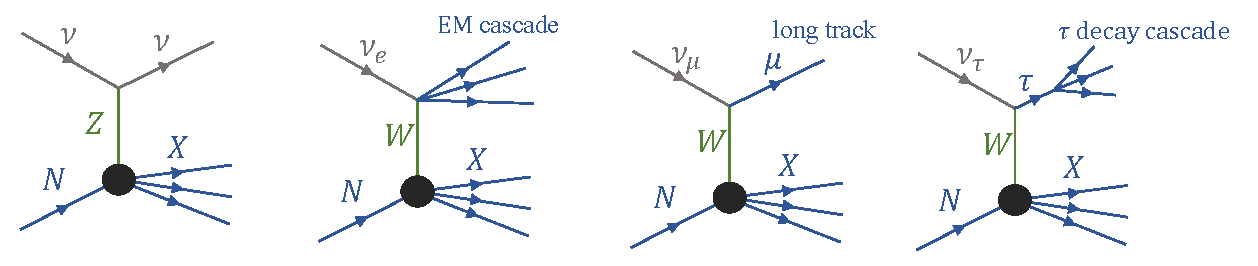
\includegraphics[width=0.95\linewidth]{img/DIS_types.pdf}
    \caption{中微子与原子核发生DIS过程的示意图}
    \label{fig:DIS_types}
\end{figure}

中微子与质子的DIS过程的总反应截面如图\ref{fig:DIS_cross_section}所示。对于中微子望远镜的研究而言,DIS的散射截面决定了其能够探测到的事件率,而反过来中微子可以通过不同入射角的中微子穿透地球的概率来估计中微子的散射截面\cite{IceCube_cross_section:2020}。对于中微子望远镜的研究来说,以下DIS散射截面的特点是比较重要的:
\begin{enumerate}
    \item 在能量比较高处($E_\nu \gtrsim 1 \,\mathrm{TeV}$),中微子和反中微子的散射截面几乎相同,而带电流的散射截面大约是中性流的两倍。
    \item 在极高能处($E_\nu \gtrsim 1 \,\mathrm{PeV}$),散射截面有如下关系$\sigma_{\nu(\bar{\nu})N} \propto E_\nu^{0.36}$。
    \item $\mathrm{Bjorken}-y$参数的平均值会随着中微子能量的增加而逐渐减小,如图\ref{fig:Bjorken_y}所示。
    \item 平均自由程大约等效于地球直径的中微子的能量大约为$40\,\mathrm{TeV}$。
\end{enumerate}

\begin{figure}[htb]
    \centering
    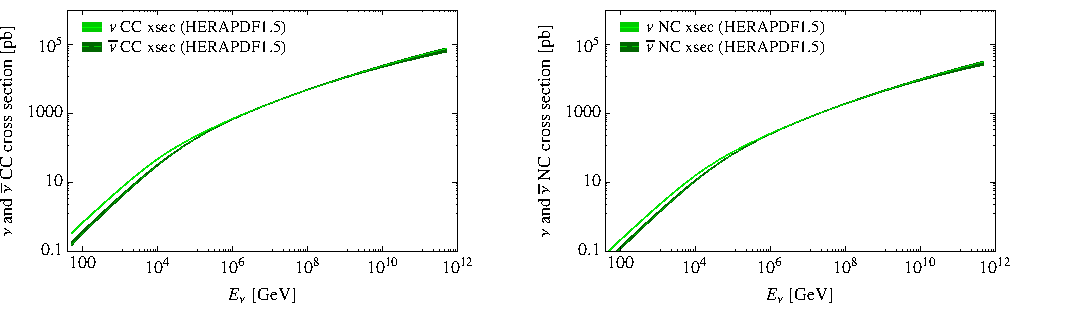
\includegraphics[width=0.95\linewidth]{img/DIS_cross_section.pdf}
    \caption{中微子与同位旋为0的原子核发生DIS过程的散射截面。左图:带电流反应;右图:中性流反应。图片来自\parencite{Sarkar_DIS:2011}}
    \label{fig:DIS_cross_section}
\end{figure}

\begin{figure}[htb]
    \centering
    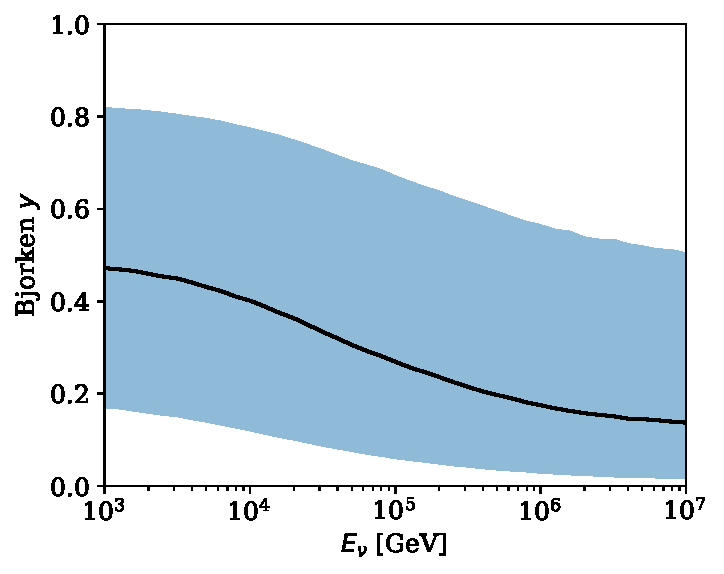
\includegraphics[width=0.7\linewidth]{img/Bjorken_y.pdf}
    \caption{$\mathrm{Bjorken}-y$与中微子能量的关系。黑线表示中位数,蓝色阴影带表示$1\sigma$范围。数据由Pythia-8.3\cite{Pythia8.2:2014, Pythia8.3:2022}模拟得到。}
    \label{fig:Bjorken_y}
\end{figure}

在能量比较低的区域,除了DIS过程外,中微子和物质的反应还包括准弹性散射(quasielastic scattering)和共振散射(resonance  production)。
在前者中,中微子可以从原子核中撞出一部分核子,而在后者中,原子被中微子激发到激发态(如$\Delta$,$N^*$)再快速衰变\cite{CS_Formaggio:2012}。
在低能处,中微子通过带电流的不同反应通道的散射截面如图\ref{fig:DIS_cross_section_le}所示。

\begin{figure}[htb]
    \centering
    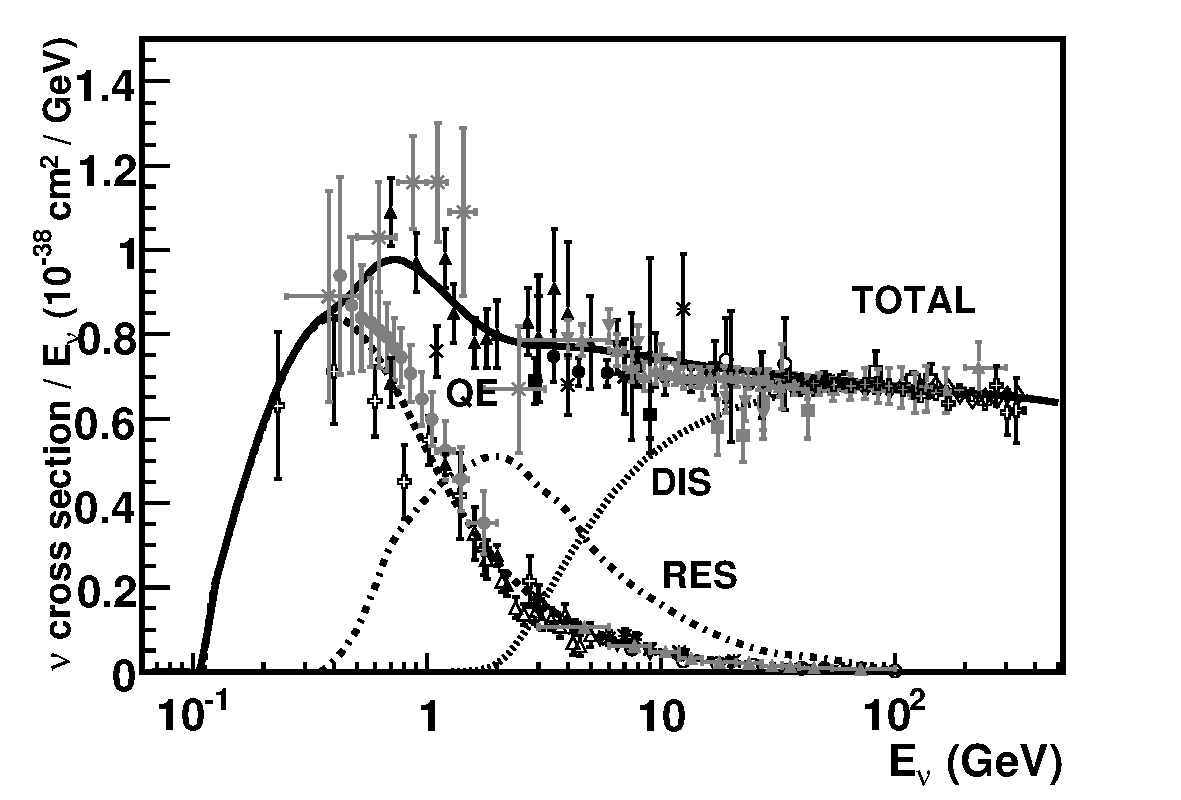
\includegraphics[width=0.45\linewidth]{img/cross_section_le_CC.pdf}
    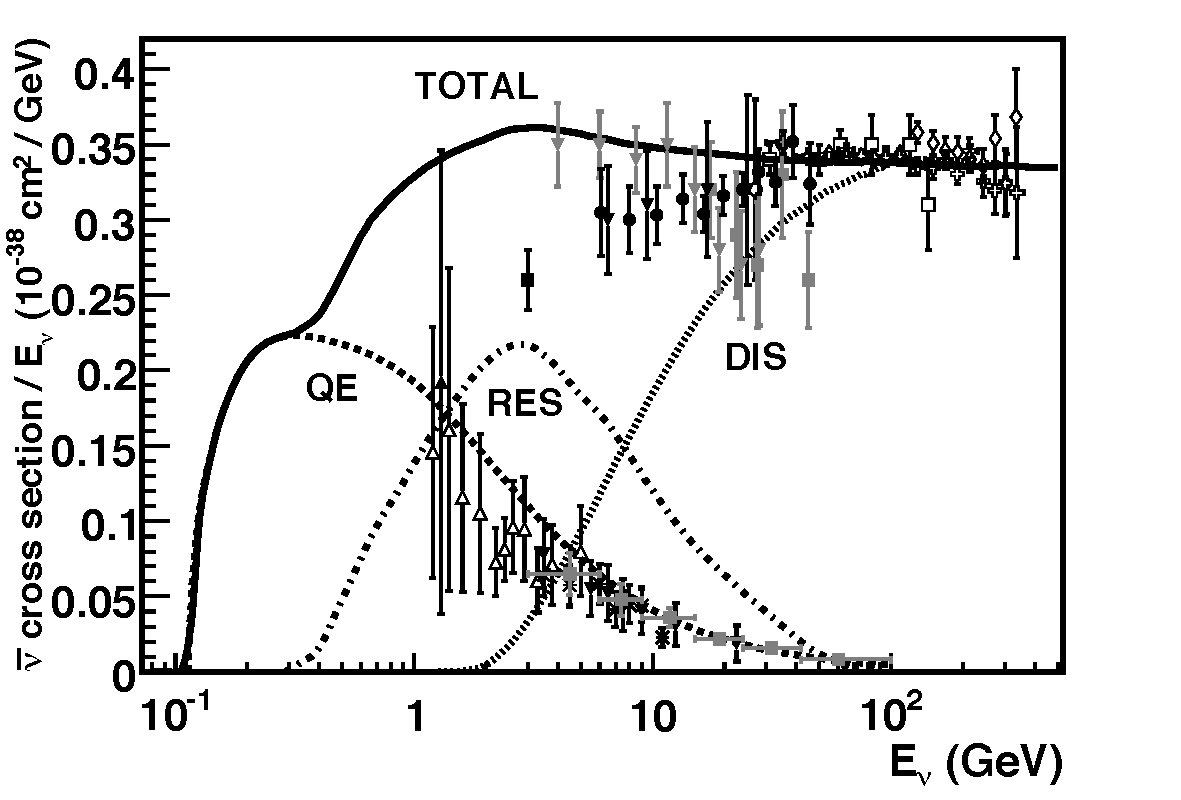
\includegraphics[width=0.45\linewidth]{img/cross_section_le_CCbar.pdf}
    \caption{低能处,中微子与原子核通过带电流的发生各种不同通道的散射截面。左图:正中微子,右图:反中微子。图片来自\parencite{CS_Formaggio:2012}}
    \label{fig:DIS_cross_section_le}
\end{figure}




\subsection{切伦科夫辐射}

\begin{figure}[htb]
    \centering
    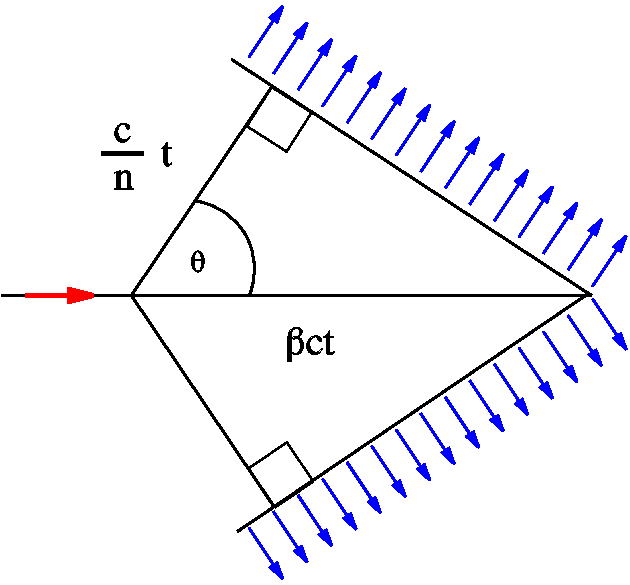
\includegraphics[width=0.4\linewidth]{img/Cherenkov_geometry.pdf}
    \caption{切伦科夫辐射的几何示意图。}
    \label{fig:Cherenkov_geometry}
\end{figure}

当带电粒子在介质中的运动速度超过介质中的光速时,便可以产生切伦科夫辐射,那是一种可以传播到远处的相干电磁辐射。
如图\ref{fig:Cherenkov_geometry}所示,切伦科夫光具有很强的方向性。切伦科夫光子与产生它的带电粒子的运动方向的夹角,即切伦科夫角$\theta_C$,满足如下关系:
\begin{equation}
    \cos \theta_\mathrm{CK}=\frac{1}{\beta n_\mathrm{p}} , 
\end{equation}
其中$\beta = v / c$是带电粒子的运动速度和光速之间的比值,$n_\mathrm{p}$表示介质的折射率。

切伦科夫光的辐射能谱可以用Frank–Tamm公式来表示:
\begin{equation}
    \frac{\mathrm{d}^2 N_\mathrm{ph}}{\mathrm{d}E_\mathrm{ph} \mathrm{d}x} = 
    \frac{2 \pi \alpha}{hc}\left(1 - \frac{1}{\beta^2 n_\mathrm{p}^2(\lambda)} \right) = 
    \frac{2 \pi \alpha}{h c} \sin^2\theta_C \simeq 
    370 \sin^2\theta_C ~\mathrm{\frac{photons}{cm \cdot eV}}
    \label{eq:Frank–Tamm}
\end{equation}
其中$\frac{\mathrm{d}^2 N_\mathrm{ph}}{\mathrm{d}E_\mathrm{ph} \mathrm{d}x}$表示在单位距离$x$中,辐射出单位能量$E_\mathrm{ph}$的光子数目$N_\mathrm{ph}$,$h$是普朗克常数。

将物理常数代入到Frank–Tamm公式并考虑到海水的折射率约为1.35以及可见光的可观测能量带约为$1\,\mathrm{eV}$(对应$350\,\mathrm{nm}$到$600\,\mathrm{nm}$的波长范围),可以得到一条简易的经验公式:一个接近光速运动的带电粒子可以在每厘米的径迹长度上产生约400个切伦科夫光子。再考虑带点粒子簇射的主要能量沉积方式为电子电离能损,而电子电离能损的强度约为$2.2\,\mathrm{MeV/cm}$。由此,我们可以得到经验公式:
\begin{equation}
    \frac{\mathrm{d} N_\mathrm{ph}}{\mathrm{d} E_\mathrm{dep}} = 
    \frac{\mathrm{d} N_\mathrm{ph}}{\mathrm{d}x} / \frac{\mathrm{d} E_\mathrm{dep}}{\mathrm{d}x} \simeq
    200 \frac{\mathrm{photons}}{\mathrm{MeV}}
    \label{eq:emission_efficiency}
\end{equation}
其中$E_\mathrm{dep}$表示高能粒子簇射在介质中沉积的能量。从这个经验关系中,我们可以得知即高能的带电粒子在海水介质中以切伦科夫光的形式辐射的光产额为$\sim 200 \mathrm{MeV}^{-1}$。

\subsection{数字光学模块}

中微子望远镜依赖于在透明介质中布置的数字光学模块(digital optical module, DOM)来探测中微子反应产生的带电次级粒子所引发的切伦科夫光信号。
以IceCube为例,它包含86根挂满DOM的根垂直探测单元(string,以下简称为串列单元),每个串列单元上挂载有60个DOM\cite{IceCube_detector:2016}。
IceCube中的DOM阵列的水平间距约为$125\,\mathrm{m}$,垂直间距为$17\,\mathrm{m}$,该阵列可以监控$1\,\mathrm{km}^3$体积的冰体。

IceCube中的使用的DOM外部是一个外直径13英寸,厚度0.5英寸的抗压玻璃球,用于保护内部的电子学设备。抗压玻璃球可以长期抵抗$250\,\mathrm{bar}$(等效于$2.6\,\mathrm{km}$的水深)的压强。
玻璃球壳要求在可见光和近紫外波段拥有高透射率,这是为了降低对本身就微弱的切伦科夫光信号的损耗。此外玻璃球壳还要求有较低的放射性背景,从而减少额外的噪声。

IceCube的DOM中包含一支日本滨松公司生产的10英寸的光电倍增管(photonmultiplier tube,PMT)\cite{IceCube_PMT:2010}。
PMT的原理如图\ref{fig:PMT_structure}所示,它借助光电效应将入射到PMT的光阴极的光子转换为光电子,并利用高压在PMT的倍增极(也称打拿级)之间产生强大的电厂,从而将电子提高电子的动能,使其在撞击下一个倍增级时能激发出更多的光子。通过多级放大,PMT可以将电子信号放大到$\mathcal{O}(10^6)$倍,这些电子最终会汇聚到阳极,产生宏观上可被观测和数字化的电流。

\begin{figure}[htb]
    \centering
    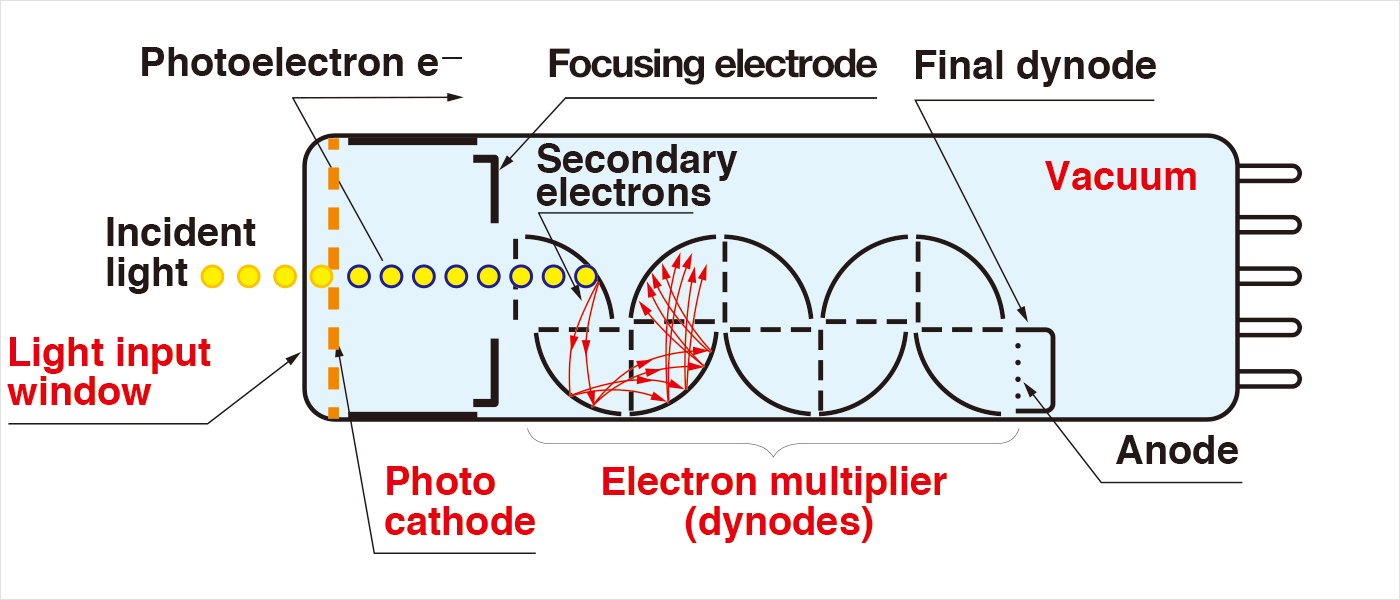
\includegraphics[width=0.85\linewidth]{img/PMT_structure.png}
    \caption{PMT的结构和工作原理示意图。图片来自\parencite{PMT_handbook:2016}}
    \label{fig:PMT_structure}
\end{figure}

PMT是非常灵敏的单光子探测设备,是中微子望远镜用来观测中微子信号的眼睛。在我们的应用中,对PMT感兴趣的主要性能参数有:

\begin{enumerate}
    \item 量子效率(quantum efficiency)。表示入射到光阴极的光子能够产生有效的光电子的概率。
    \item 增益(gain)。表示光电子在经过了多个倍增级放大之后,最终在阳极处的电子数量,即电子数量的放大率。
    \item 单光子波形(single photoelectron waveform)。表示单个光子产生的电压波形信号的形状。通常用波形的高度,上升时间和下降时间等量来表征。
    \item 单光子分辨率(single photoelectron resolution)。用于表示PMT分辨单光子信号和零光子背景噪声的能力,通常用光电子电荷量分布图中的单光子峰与零光子峰之间的峰谷比来表征。
    \item 渡越时间弥散(transient time spread)。渡越时间表示由电子在经过多个倍增极后最终到达阳极形成电流所需要的时间。而渡越时间弥散便表示电子在放大和穿行的这段时间的不确定度,它最终会体现在PMT产生的电压波形信号的上升沿时间点的弥散。
\end{enumerate}

为了避免玻璃球-空气-PMT之间由于折射率不同所带来的界面效应而引发的光子损耗,IceCube在玻璃球壳和PMT中间填充了光学胶。光学胶需要在我们的探测光的波段范围内具有高透光性($>90\%$),并且拥有$\gtrsim 1.4$的折射率,接近于玻璃的$\sim 1.5$折射率。
对于IceCube这种装备单个大英寸的PMT的DOM而言,其PMT中电子倍增放大的过程会受到地球磁场的影响,因此还需要在PMT外围包裹一层金属网罩来屏蔽地球磁场的影响\cite{pmt_Earth_magnetic:2011}。

在通过PMT将光信号转换为电信号后,需要前端读数电路将光电子的模拟信号数字化。IceCube的读数电路具有波形读出的能力,即将连续的光电子电压波形采样成离散的数据点,如图\ref{fig:IC_waveform}所示\cite{IceCube_DAQ:2008}。
IceCube拥有两种不同时间精度的波形采样设备:精度较高的是两块ATWD(Analog Transient Waveform Digitizer)芯片,它们拥有$300\,\mathrm{MHz}$的采样频率和$10\,\mathrm{bit}$的采样精度,但只能连续采样128个数据点,即连续采样$428\,\mathrm{ns}$的波形数据;精度较低的是fADC(fast Analog Digital Converter)\footnote{尽管名字中带有fast,但是$40\,\mathrm{MHz}$的采样频率在2020年代已经相对比较慢了。},它拥有$40\,\mathrm{MHz}$的采样频率和$10\,\mathrm{bit}$的采样精度并且可以连续256个数据点,即采样时间可以达到$6.4\,\mathrm{\mu s}$,足以包含绝大多数的中微子事件以及其后脉冲。

IceCube中的ATWD不同于可以连续采样的ADC,是一种SCA(Switched Capacitor Arrays)。它通过先将电压信号储存在电容器阵列中,再利用相对低速的ADC从电容阵列中读取电压值的形式,从而在低功耗的情况下实现高时间精度的采样\cite{DRS4:2010}。
ATWD的应用帮助IceCube在2000年代便达到了$300\,\mathrm{MHz}$的信号采样频率,为分析中微子信号提供了有力的支撑。这些高精度的波形信号还可以被用于寻找陶中微子所对应的双峰波形结构,提高了IceCube对中微子味道的分辨能力\cite{IceCube_tau_Donglian:2015, IceCube_tau_Logan:2019, IceCube_tau:2020}。
SCA技术路线的弊端是需要等待低速ADC读取电压,因而会有比较长的死时间。以IceCube中的ATWD为例,死时间有$29\,\mu\mathrm{s}$,因此IceCube设计了双ATWD芯片的备用机制,用于应对时间上紧密相邻的信号。

在新一代的中微子望远镜中,人们开始尝试在数字光学模块中使用多个小型的PMT来代替单个大型的PMT。
例如KM3NeT中采用了一个mDOM(multi DOM)的探测模块,每一个玻璃球内都包含有31个具有独立采数通道的PMT,通过对要求同时有多个PMT接收到光子信号,可以有效避免PMT自身的暗噪声以及海水的光学噪声背景的影响\cite{KM3NeT_mDOM:2014, KM3NeT_mDOM:2015, KM3NeT_mDOM:2022}。
IceCube-Gen2中也计划使用包含多个PMT的mDOM\cite{IceCube-Gen2_mDOM:2021}。
这些有关新光学模块的技术将会在一个中间项目——IceCube-upgrade\cite{IceCube-upgrade:2019}中进行研究和测试\cite{IceCube_upgrade_mDOM:2021, IceCube_D-Egg:2022}。
我们团队也有进行新型数字光学模块的设计,我们提出了hDOM(hybrid DOM)\cite{hDOM:2021}的设计构想,即在一个模块中即加入PMT又加入SiPM,从而提高模块的时间分辨率和感光面积。hDOM的设计和优势将会在章节\ref{sec:hdom}中具体介绍。

除了对光敏元件进行改造外,新一代的中微子望远镜还会采用更加现代化的电子学设计。
近10年来的数字电路数字电路部分则发生了天翻地覆的变化,我们需要着重考虑采用这些新型的技术,例如小白兔时钟同步\cite{white_rabbit:2013},性能更好的高速ADC\cite{Changda_PandaX_ADC:2021},通过更加强大的FPGA芯片来实现复杂的后端采数和触发的算法等。

\begin{figure}[htb]
    \centering
    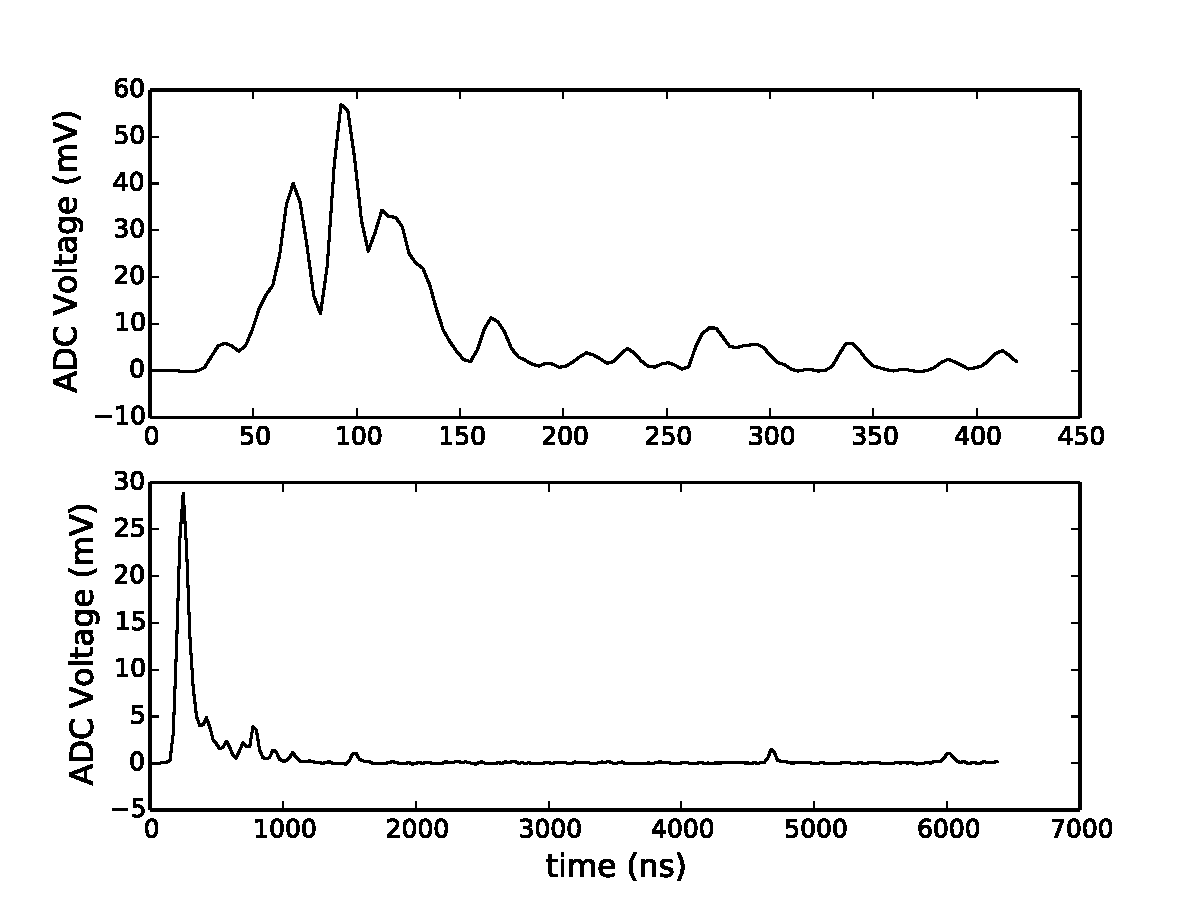
\includegraphics[width=0.8\linewidth]{img/IC_waveform.pdf}
    \caption{IceCube中对PMT产生的光电子电压信号采样得到的波形。图片来自\parencite{IceCube_detector:2016}}
    \label{fig:IC_waveform}
\end{figure}

\begin{figure}[htb]
    \centering
    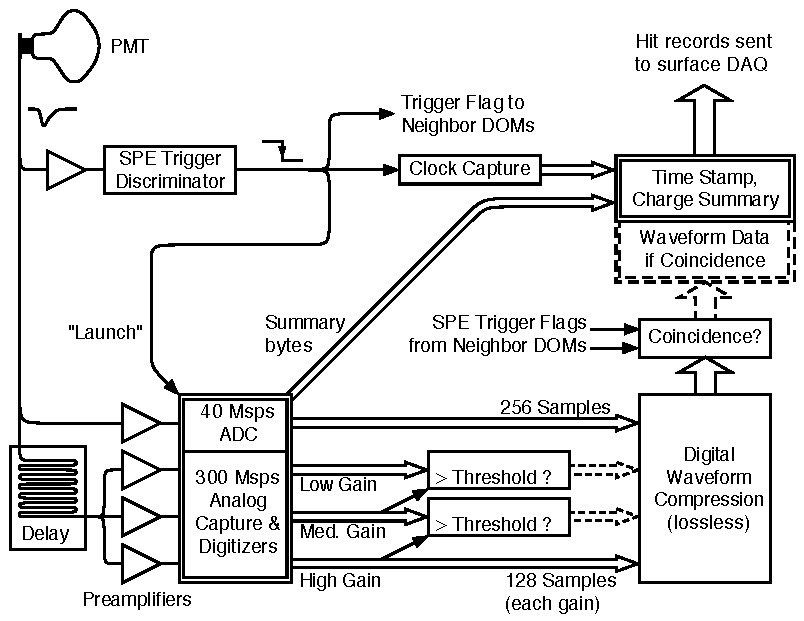
\includegraphics[width=0.8\linewidth]{img/IC_DOM_data_flow.pdf}
    \caption{IceCube中DOM对PMT采集到的信号进行数字化的流程图。图片来自\parencite{IceCube_detector:2016}}
    \label{fig:IC_DOM_data_flow}
\end{figure}

\subsection{中微子事件类型}

如图\ref{fig:DIS_types}中所示,不同味道和不同反应通道的中微子发生DIS的产物不同,最终在DOM阵列中观测到的事件形态也有所不同,通常人们将中微子事件分为以下三种类型:
\begin{enumerate}
    \item 径迹型事件(track event):由缪子中微子通过带电流通道产生的缪子所产生的事件类型。
    \item 簇射型事件(cascade event):由电子中微子通过带电流流通道产生的的电子,或者所有味道的中微子通过中性流通道产生的强子簇射所产生的事件类型。
    \item 双簇射型事件(double-cascade event)由陶中微子通过带电流产生陶子的同时形成强子簇射,以及陶子衰变产生簇射,所组合而成的事件类型。
\end{enumerate}

\begin{figure}[htb]
    \centering
    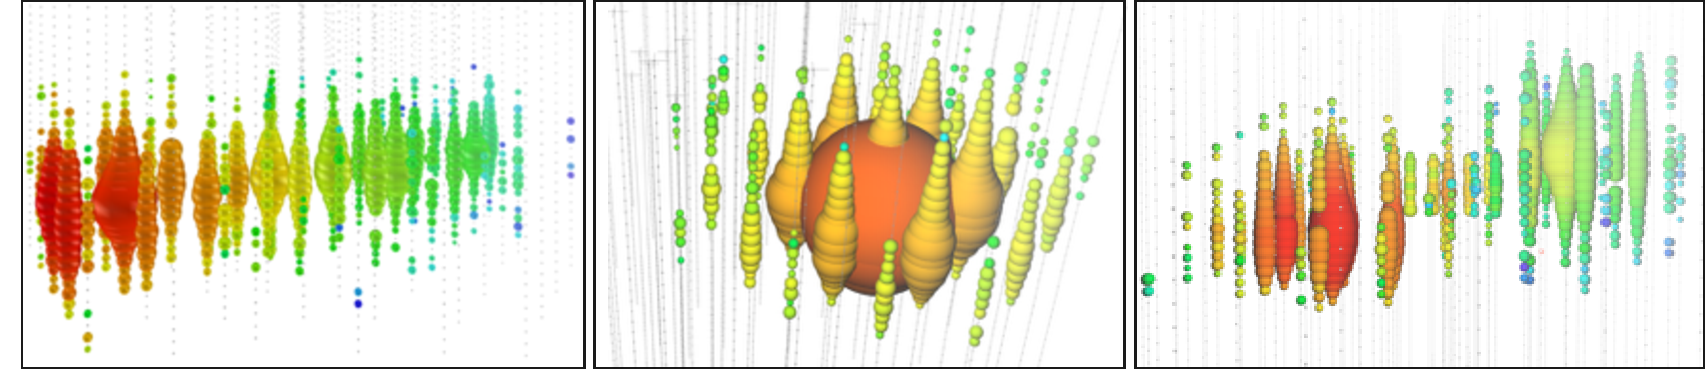
\includegraphics[width=0.98\linewidth]{img/event_topologies.pdf}
    \caption{IceCube模拟得到的DOM观测到的不同形态的中微子事件。左图对应径迹型事件,中图对应簇射型事件,右图对应双簇射型事件。图中每一个有颜色的点表示DOM观测到了来自中微子事件的光子,其颜色表示光子到达时间,大小表示DOM接收到的光子数量。图片来自\parencite{IceCube-Gen2_white_paper:2020}}
    \label{fig:event_topologies}
\end{figure}


这些不同类型的中微子的形态特征如图\ref{fig:event_topologies}所示。由缪子中微子产生的缪子能够在介质中穿行数公里,形成鲜明的径迹型事件。这种事件通常可以重建得到最好的角度分辨能力\cite{AMANDA_track_reco:2003, IceCube_track_reco:2021, KM3NeT_reco:2017, Baikal_track_reco:2021},因而常被用于寻找中微子的天体物理起源\cite{IceCube_10yr_point_source:2019, KM3NeT_sensitivity:2018, ANTARES_IceCube_point_source:2020}。
但这种事件有比较高的背景,因为宇宙线轰击大气形成簇射的过程中也会产生缪子和中微子,在探测器阵列中产生径迹型事件。
在IceCube所处的深度,这些大气缪子的流量在$\mathrm{TeV}$能级处大约是天体物理起源中微子的流量的$\mathcal{O}(10^4)$倍\cite{IceCube_atmos_muon_flux:2018}。因此在数据分析时,人们通常选用来自地心那一侧或者能量比较高的径迹型事件,来减少大气缪子和大气中微子的干扰的影响。

另外一种有效去除大气缪子背景的方式是在径迹型事件和簇射型事件中进一步选取初始径迹型事件(starting-track event)\cite{IceCube_starting_track:2021}。
在这种事件中,缪子中微子与原子核DIS反应的顶点就发生在探测器内部,因而可以和来自大气中并且会经过探测器阵列外围的DOM的缪子背景进行区分。
同时这种方法可以通过屏蔽与大气缪子在时间上成协的信号来降低大气中微子的噪声\cite{IceCube_atmos_neutrino_flux:2016}。
但是由于在事件筛选和方向重建方面的困难以及事件样本数量的缺少,这种信号通道并没有得到大规模的应用\cite{IceCube_starting_track:2021b}。

簇射型事件通常拥有更好的能量分辨率\cite{IceCube_energy_reco:2013, KM3NeT_reco:2017, Baikal_cascade_reco:2022},可以用于很好地测量天体物理中微子的流强\cite{IceCube_6yr_cascade_spectrum:2020}。
在IceCube中,由于簇射型事件的角度重建精度比较差\cite{IceCube_cascade_dir_reco:2019, IceCube_cascade_dir_reco:2021},一般为10度左右,故较少用于做中微子的点源搜寻\cite{IceCube_cascade_source_search:2016}。
而在水基的望远镜中,例如KM3NeT和Baikal-GVD,由于深水的散射要远小于冰中的散射\cite{OP_ANTARES:2004, OP_Baikal:2012, OP_Grace:2018, OP_IceCube:2006, OP_NEMO:2006, OP_P-One:2021},故可以对簇射型事件进行较好的方向重建,其重建精度可以达到几度的水平\cite{KM3NeT_reco:2017, Baikal_cascade_reco:2022},在这种情况下,簇射型事件也可以被用于做多信使方面的研究\cite{Baikal_cascade_events:2019, Baikal_TXS:2022}。

双簇射型事件只能通过陶中微子的带电流作用产生,因此它可以用于寻找陶中微子\cite{IceCube_tau_Donglian:2015, IceCube_tau_Logan:2019, IceCube_tau:2020, Baikal_double_cascade_tau:2023, KM3NeT_double_cascade_tau:2021}。
双簇射型事件的第一个簇射是原子核被中微子DIS过程击碎后产生的强子簇射,第二个簇射是陶轻子衰变产生的电磁簇射($18\%$)或者强子簇射($\sim 65\%$)。而在剩余的衰变通道($17\%$)中,陶轻子衰变产生一个缪子,形成与初始径迹型事件类似的事件形态。

陶轻子的寿命$t_\mathrm{decay} = 3\times10^{-13} \,\mathrm{s}$非常地短暂,但是在洛伦兹变化下,高能的陶轻子在实验室系下的时间流逝速度会变缓,因而可以飞行比较长的距离。陶轻子在衰变前的飞行距离$l_\tau$和陶轻子能量$E_\tau$由如下关系:
\begin{equation}
    l_\tau = \frac{E_\tau}{m_\tau} \times c t_\mathrm{decay} \simeq 50\,\mathrm{m} \times \frac{E_\tau}{1\,\mathrm{PeV}} ,
    \label{eq:tau_decay}
\end{equation}
其中$c$为光速,而$m_\tau=1.776 \,\mathrm{GeV}$为陶轻子的质量。考虑到探测器对簇射顶点的重建精度约为$3\,\mathrm{m}$,而且单个高能簇射在纵向上的尺度约为$10\,\mathrm{m}$,因此只有能量达到$\gtrsim 100 \, \mathrm{TeV}$的陶中微子事件才能产生容易分辨的双簇射型信号。

双簇射型事件除了可以从几何特征的上寻找外\cite{IceCube_tau:2020},还可以根据时间特征来寻找。
这两个簇射在到达DOM的时间上存在一定的先后关系,因而会在PMT的波形上形成双脉冲的结构,用时间方法寻找到的陶中微子事件也被称为双脉冲型事件\cite{IceCube_tau_Donglian:2015, IceCube_tau_Logan:2019, Tian_tau_double_pulse:2021}。
这两种测量方法分别对中微子望远镜阵列的空间和时间分辨能力有一定的要求。

\section{台址选择}

\subsection{介质的光学性质}

海水的光学性质,主要指海水的吸收长度和散射长度。光学性质决定了中微子望远镜所探测到的切伦科夫光信号的强度和质量,进而对望远镜探测的能量阈值,角分辨率等性能都有重要的影响,是在设计望远镜阵列的几何排布时要考虑的主要因素。
因此,几乎所有的望远镜都会对选址处的光学性质开展原位的测量和分析\cite{OP_ANTARES:2004, OP_Baikal:2012, OP_Grace:2018, OP_IceCube:2006, OP_IceCube:2013, OP_NEMO:2006, OP_P-One:2021}。

\subsection{纬度位置}

与光学和射电的望远镜类似,中微子望远镜也拥有一段最灵敏的探测区域,我们称之为灵敏带。
中微子望远镜对来自水平方向上的中微子流强拥有最好的灵敏度,这是因为在水平方向上的屏蔽层柱密度的大小适中,即能保证将大气缪子全部吸收,又不至于吸收高能的中微子事件。

中微子望远镜所处的纬度位置决定了它的灵敏带能够覆盖的天区范围,如图\ref{fig:detector_poistion_and_sensitive_band}中所示。
位于南极的IceCube的灵敏带在赤道坐标系下是一条水平的环带,由于IceCube坐落在南极点,因此它和它的灵敏带都不会随着地球的转动而发生转动。
位于其他区域的中微子望远镜的灵敏带会随着地球的自转扫过不同的天区,特别的,靠近赤道上的中微子望远镜的灵敏带能够扫过整个天区。
坐落在地球不同位置的中微子望远镜可以形成互补的大型高能中微子观测网络\cite{PLENuM:2021},其灵敏带能够覆盖全天各个方向的中微子源。


\begin{figure}[htb]
    \centering
    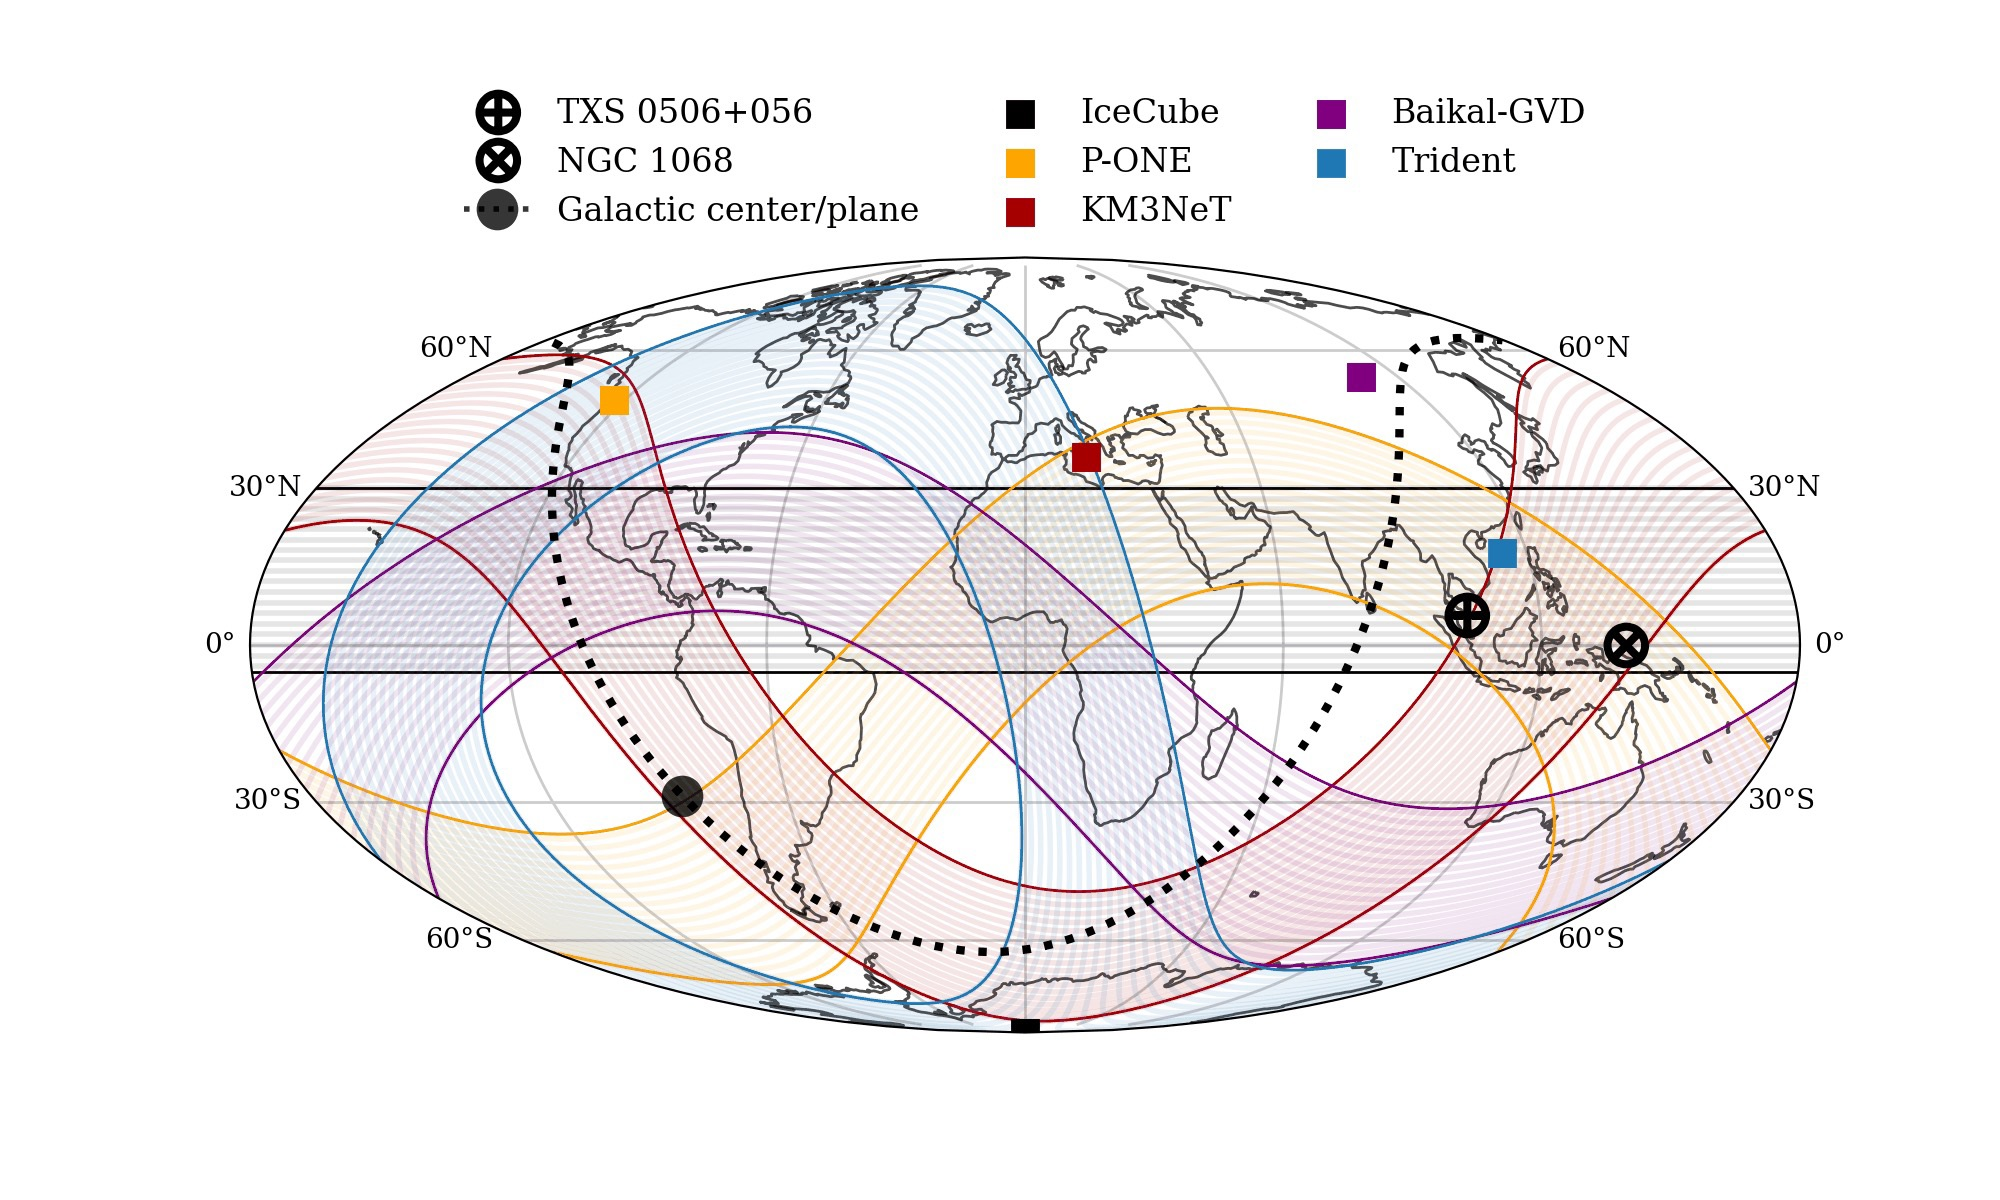
\includegraphics[width=0.95\linewidth]{img/detector_poistion_and_sensitive_band.jpg}
    \caption{目前已经建成或者规划中的中微子望远镜的位置以及其灵敏带。图片由Lisa Schumacher制作,截取自报告\cite{LuLu_PeVPA:2022}}
    \label{fig:detector_poistion_and_sensitive_band}
\end{figure}


\subsection{其他因素}

除了上文中介绍的两点以外,还有其他地理和环境的因素会对中微子望远镜产生影响,例如:

\begin{enumerate}
    \item 海水深度。中微子望远镜依赖于海水来屏蔽日光和大气缪子背景。太阳光在$\sim 1\,\mathrm{km}$的深度之后便已经被完全屏蔽。而对于大气缪子背景而言,海水的厚度每增加$1\,\mathrm{km}$,大气缪子的流量便会下降约一个数量级\cite{atmos_muon_depth:1998, KM3NeT_atmos_muon:2019}。此外海水的深度还会影响洋流和生物丰度等。

    \item 洋流流速和均匀性。洋流会使得中微子阵列中的串列单元的位置偏离预设位置,对串列单元的力学性能提出要求。通过海底声学系统,可以对DOM的位置进行$\lesssim 10\, \mathrm{cm}$级别的定位\cite{KM3NeT_acoustic_1:2022, KM3NeT_acoustic_2:2022, Baikal_acoustic:2021},从而消除一部分洋流的影响。洋流在阵列尺度上的均匀性也是需要考虑的要点。海洋的洋流存在中小尺度的涡旋结构(公里级到亚公里级)\cite{current_simulation:2017},这种涡旋可能会改变阵列的形状结构,甚至使串列单元之间发生缠绕。

    \item 生物丰度。深海鱼类会通过发出光信号来进行相互之间的交流,此外海水中的有机物大分子也会在受到扰动之后(例如随着洋流碰撞到DOM上)发出生物光\cite{biolumi_modeling:2021}。这些信号对于中微子望远镜来说是一大主要的噪声干扰\cite{ANTARES_biolumi:2021, Baikal_biolumi:2021}。
\end{enumerate}

\section{世界上的中微子望远镜}

\subsubsection*{DUMAND}

\begin{figure}[htb]
    \centering
    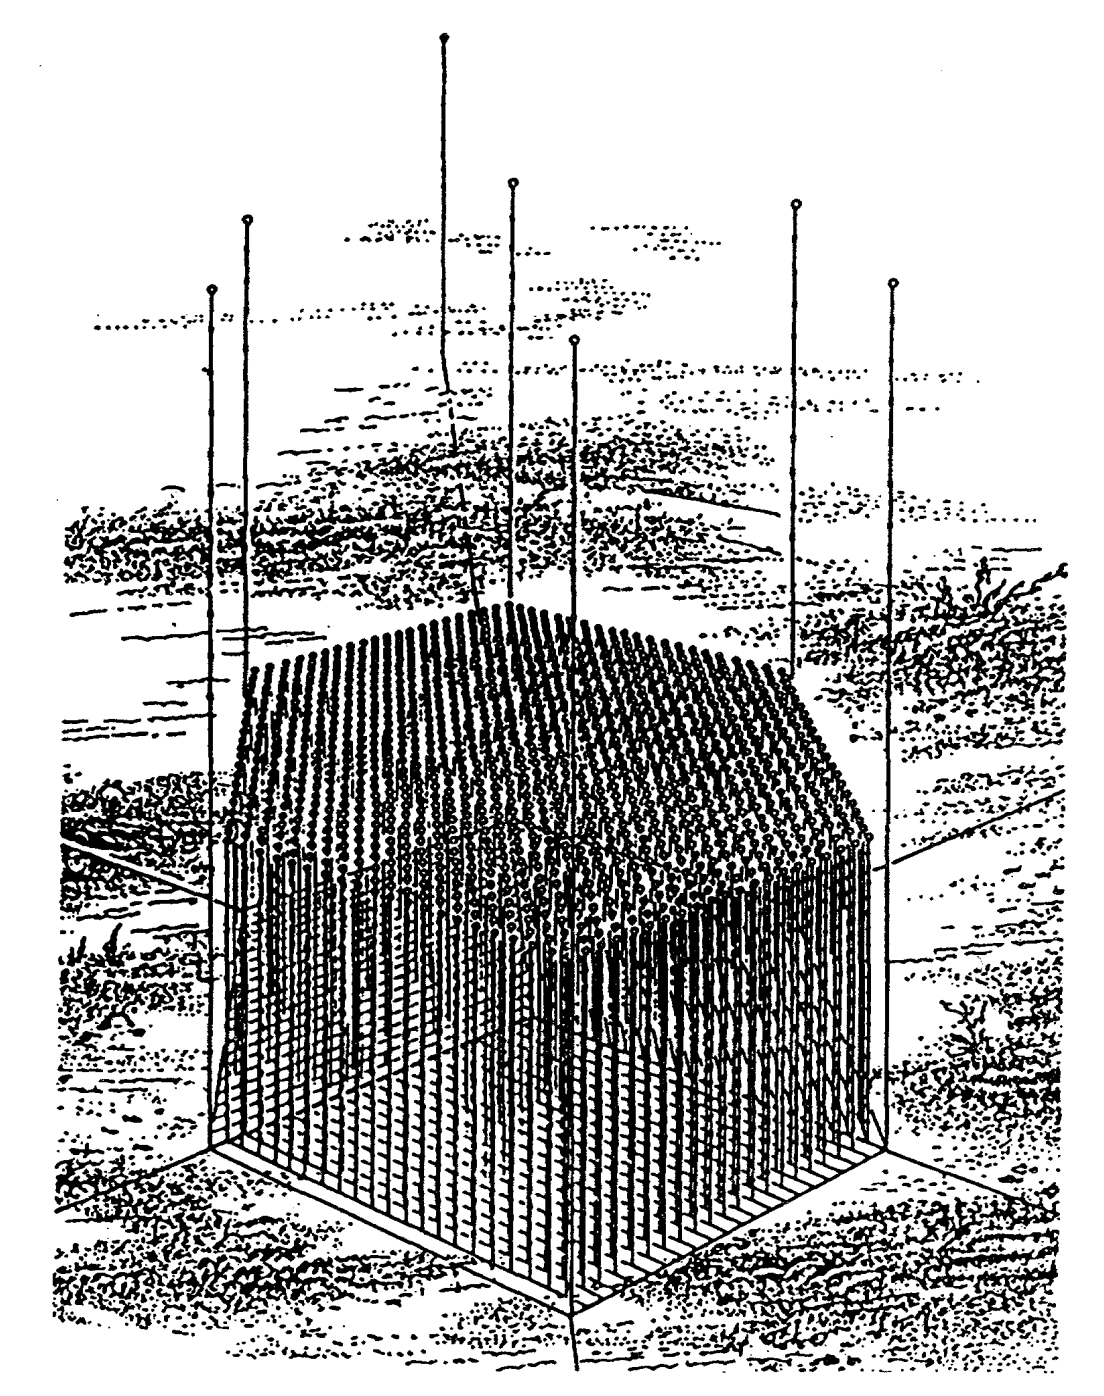
\includegraphics[width=0.65\linewidth]{img/DUMAND.png}
    \caption{DUMAND阵列设计图。图片来自\parencite{DUMAND:1992}}
    \label{fig:DUMAND}
\end{figure}

DUMAND\cite{DUMAND:1992}是第一台正式地进行详细设计并投入建设的大型中微子望远镜。它选址于夏威夷岛附近$\sim 4 \,\mathrm{km}$深的海底,计划构建世界上第一个$\sim\mathrm{km}^3$级大小的光敏探测阵列,如图\ref{fig:DUMAND}所示。然而受限于当时的海洋工程技术,DUMAND-II项目在布放第一根串列单元便遇到了线缆通讯的故障,最终被美国能源部终止\cite{Telescope_history:2019}。
尽管没有成功建设成大型阵列,DUMAND合作组在长达20多年的时间中,对中微子望远镜的探测原理,科学目标,工程设计等等内容都进行了充分的探讨,为后世其他中微子望远镜的建设奠定了基础\footnote{\url{https://www.phys.hawaii.edu/~dumand/dumacomp.html}}。

\subsubsection*{AMANDA}

AMANDA\cite{AMANDA:1999}实验位于南极的冰川冰中,它成功地在$1150\,\mathrm{m}$~$2350\,\mathrm{m}$米的冰层中布置了约700个光敏探测阵列,如图\ref{fig:AMANDA}所示。
然而由于AMANDA的阵列规模较小,以及其光敏元件中缺乏数字化模块,AMANDA并没有找到高能的天体中微子信号\cite{AMANDA_neutrino_search:2007}。

\begin{figure}[htb]
    \centering
    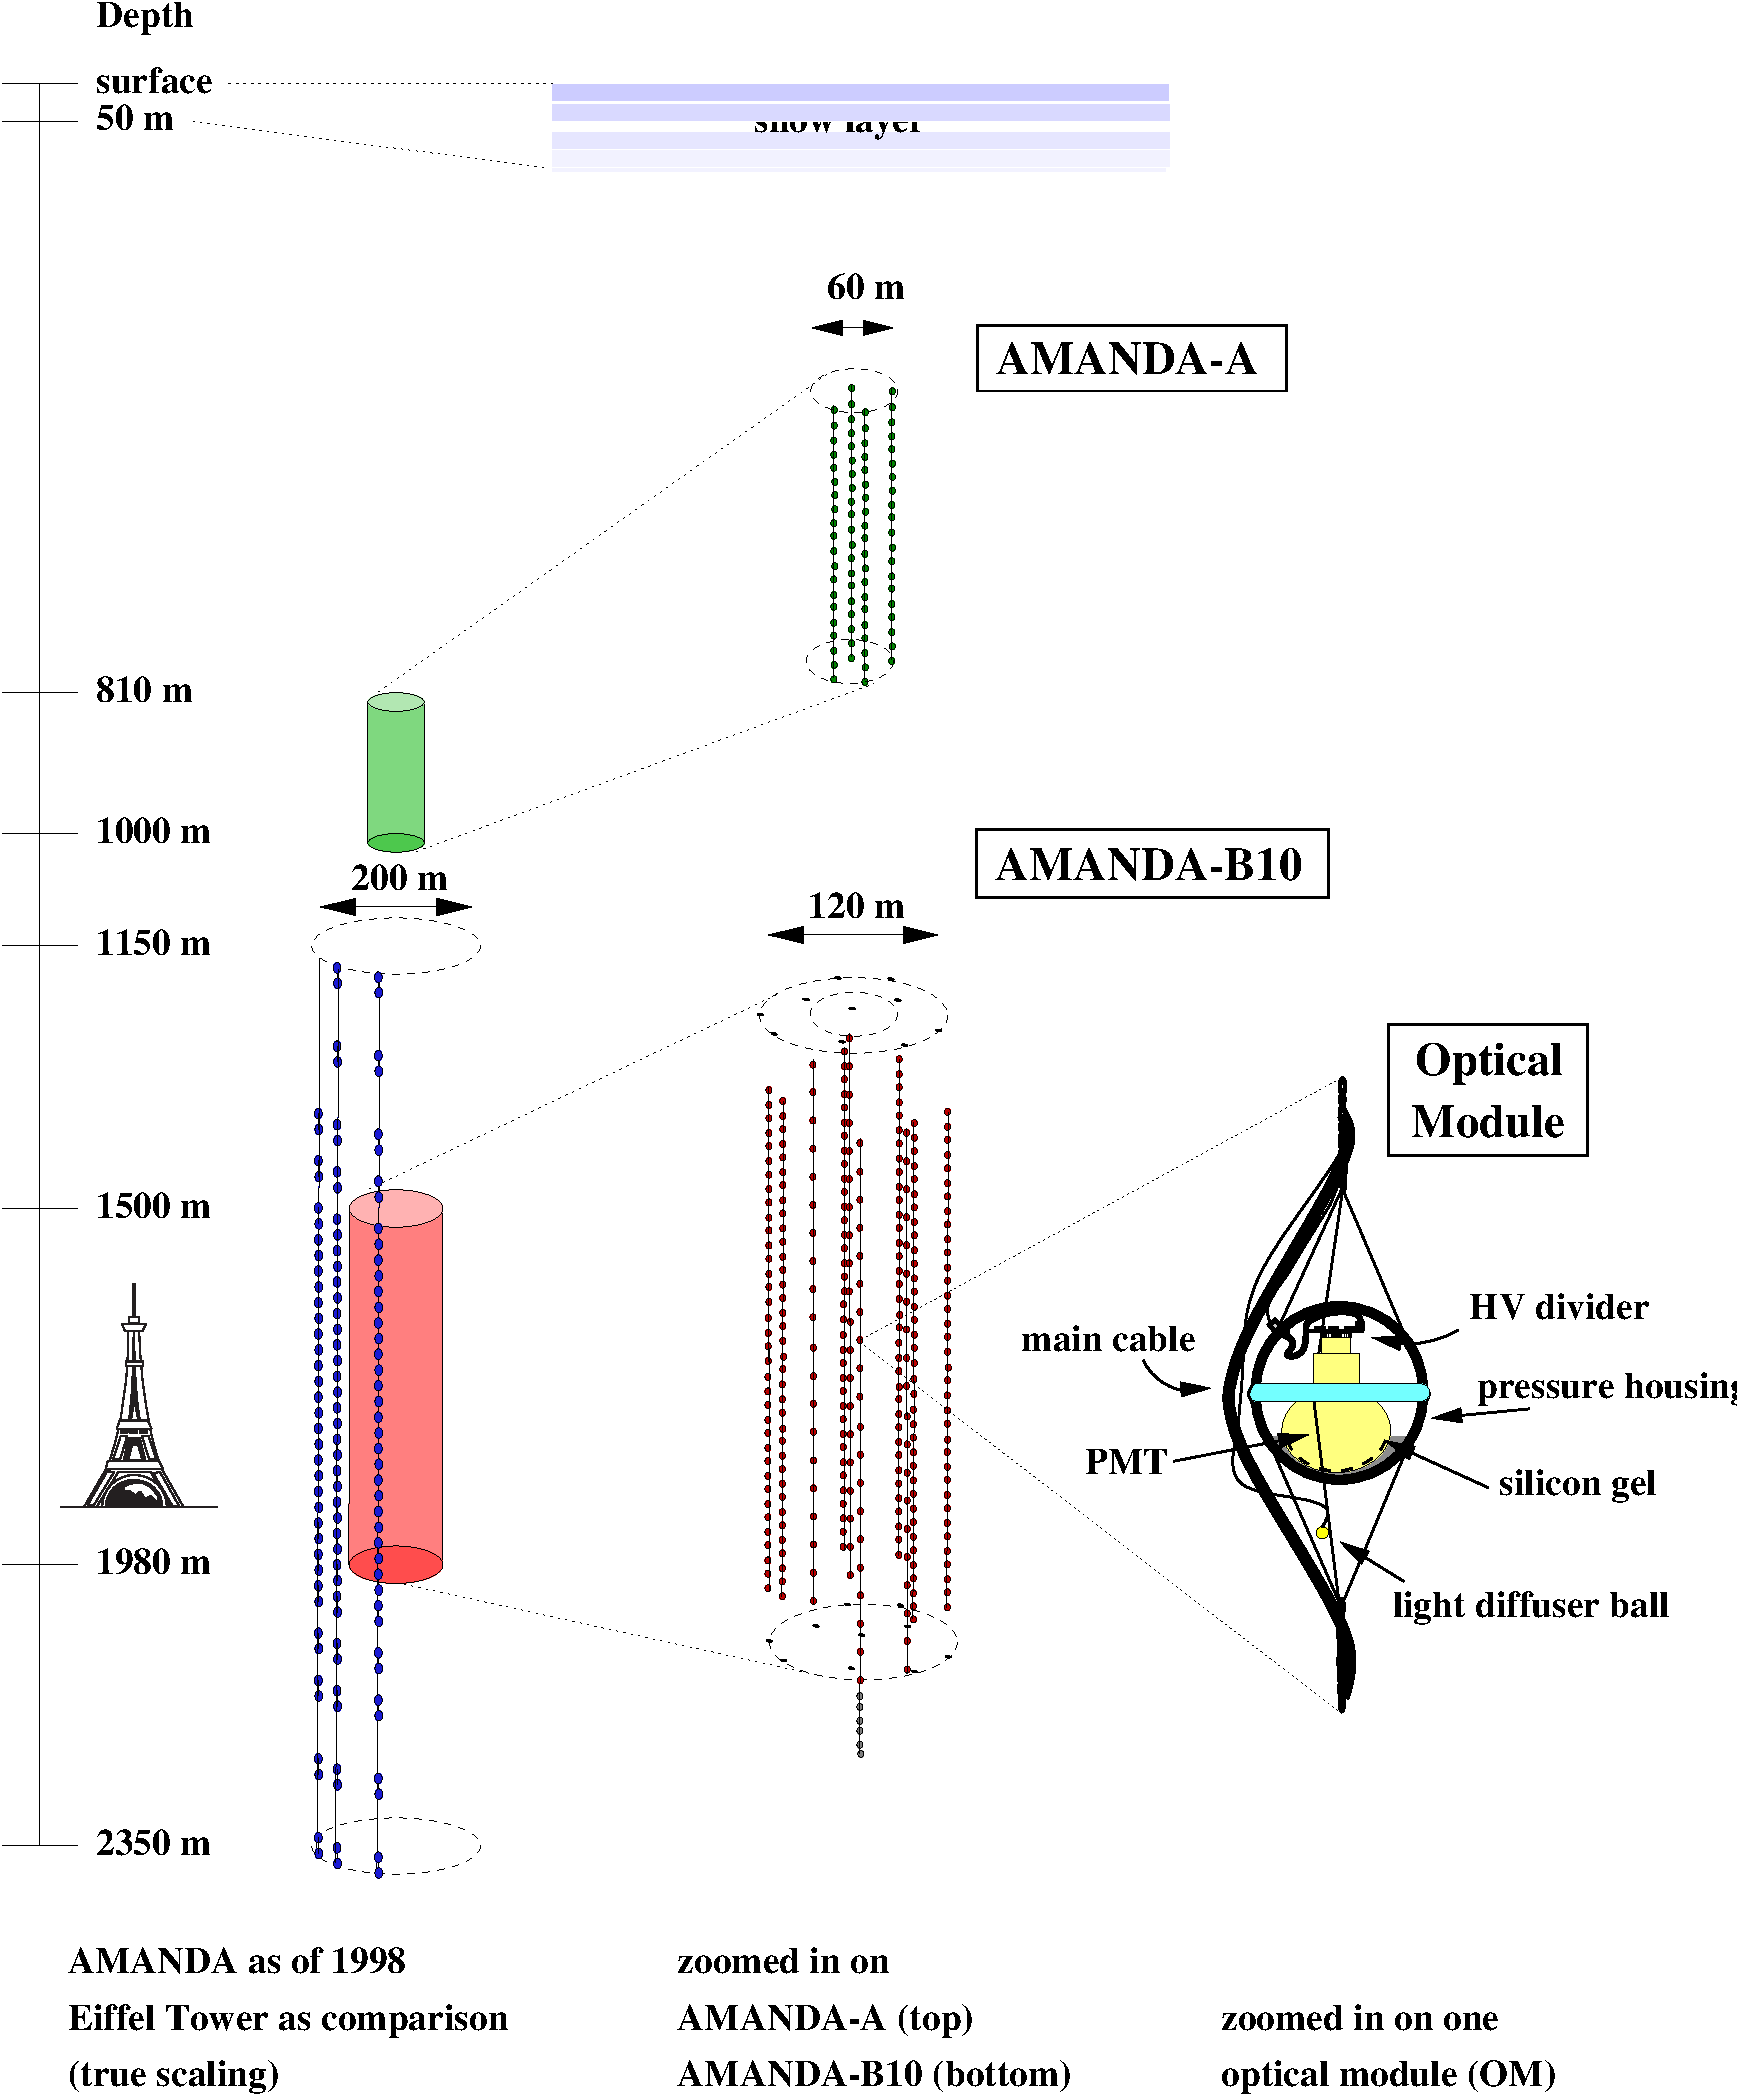
\includegraphics[width=0.75\linewidth]{img/AMANDA.pdf}
    \caption{AMANDA阵列设计图。图片来自\parencite{AMANDA:1999}}
    \label{fig:AMANDA}
\end{figure}

\subsubsection*{Antares}

Antareas中微子望远镜位于法国南部2800米深的海水中,由约900个DOM组成\cite{ANTARES:2011}。
它是第一台真正建成的深海中微子望远镜,自2008年建成以来,它很多年的时间内保持了北半球最灵敏的中微子望远镜的地位\cite{ANTARES_highlights:2022}。
尽管没有显著地探测到高能的天体中微子,它的实验设计为后续的KM3NeT项目提供了不少经验。

\subsubsection*{IceCube}

IceCube是AMANDA的继承项目,它是世界上首个达到$1\,\mathrm{km^3}$体积的中微子望远镜,也是观测成果最为丰硕的望远镜\cite{IceCube_detector:2016}。IceCube在南极冰层下1450米到2450米之间布置了86根串列单元,每根上面挂载60个DOM,其阵列的示意图如图\ref{fig:IceCube_array}所示。
IceCube的阵列中DOM之间垂直间距为$16.7\,\mathrm{m}$,水平间距为$125\,\mathrm{m}$,这种悬殊的间距比例是由于IceCube在南极布置串列单元时需要支付昂贵的燃料费用于融化冰川冰。

除了冰层下的光学阵列外,IceCube在冰层上还有能够观测宇宙线阵列的地面阵列——IceTop\cite{IceTop:2012}。它可以与冰层中的光学阵列一同实现对宇宙线簇射中缪子的测量,从而有效地测量$1\,\mathrm{PeV}$到$1\,\mathrm{EeV}$的宇宙线成份\cite{IceTop_measurement:2013},并且可以帮助屏蔽IceCube屏蔽一部分大气缪子的干扰。

\begin{figure}[!htb]
    \centering
    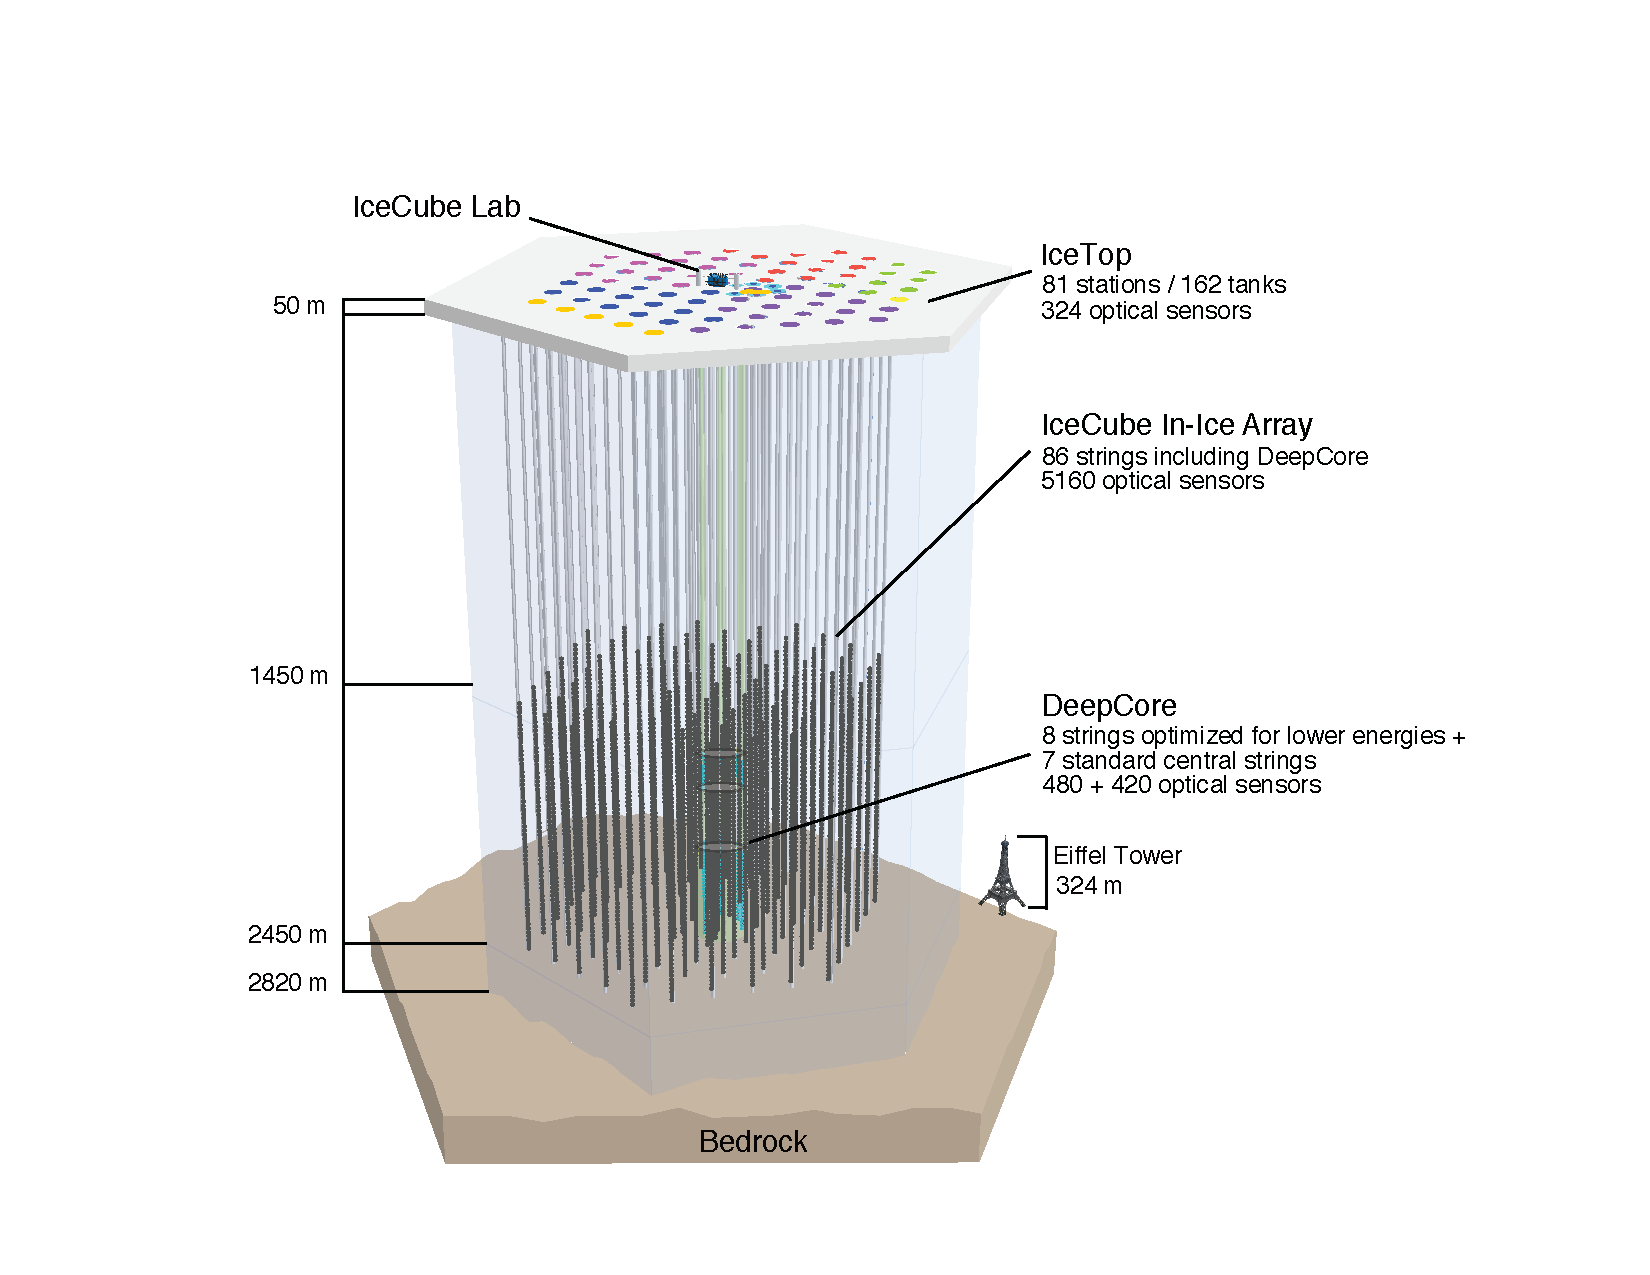
\includegraphics[width=0.8\linewidth]{img/IceCube_array.pdf}
    \caption{IceCube阵列设计图。图片来自\parencite{IceCube_detector:2016}}
    \label{fig:IceCube_array}
\end{figure}

\subsubsection*{Baikal-GVD}

贝加尔湖是世界上最大的淡水湖,其水深可以达到$1500\,\mathrm{m}$,足以容纳一个中微子望远镜。贝加尔湖在冬季湖水表面上会结上一层超过1米厚的冰层,而在冰层上施工相比于大洋上施工会有诸多的便利。
贝加尔湖上曾经诞生过多个中微子望远镜项目,例如早期的NT-36,NT-200\cite{NT_200:1997},以及目前正在建造的Baikal-GVD\cite{BAIKAL_design:1997}。

如图\ref{fig:Baikal_scope}中所示,Baikal-GVD阵列由多个探测区块组成,目前已经完成了8个探测区块的建设,每一个探测区块之间的距离为$200\,\mathrm{m}$到$300\,\mathrm{m}$之间,其整体的监控体积达到$0.6\,\mathrm{km^3}$,是目前北半球最灵敏的中微子望远镜。
Baikal-GVD的每一个探测区块包含8根串列单元,形成一个半径$60\,\mathrm{m}$,高$525\,\mathrm{m}$的圆柱体。Baikal-GVD的每一根串列单元上包含了36个光敏元件,它们的深度位于$750\,\mathrm{m}$到$1275\,\mathrm{m}$之间,垂直间距约为$15\, \mathrm{m}$。
这些光敏元件并不具备数字化的功能,而是将模拟信号传输到附近的专门用于数字化的球舱内来处理。

\begin{figure}[!htb]
    \centering
    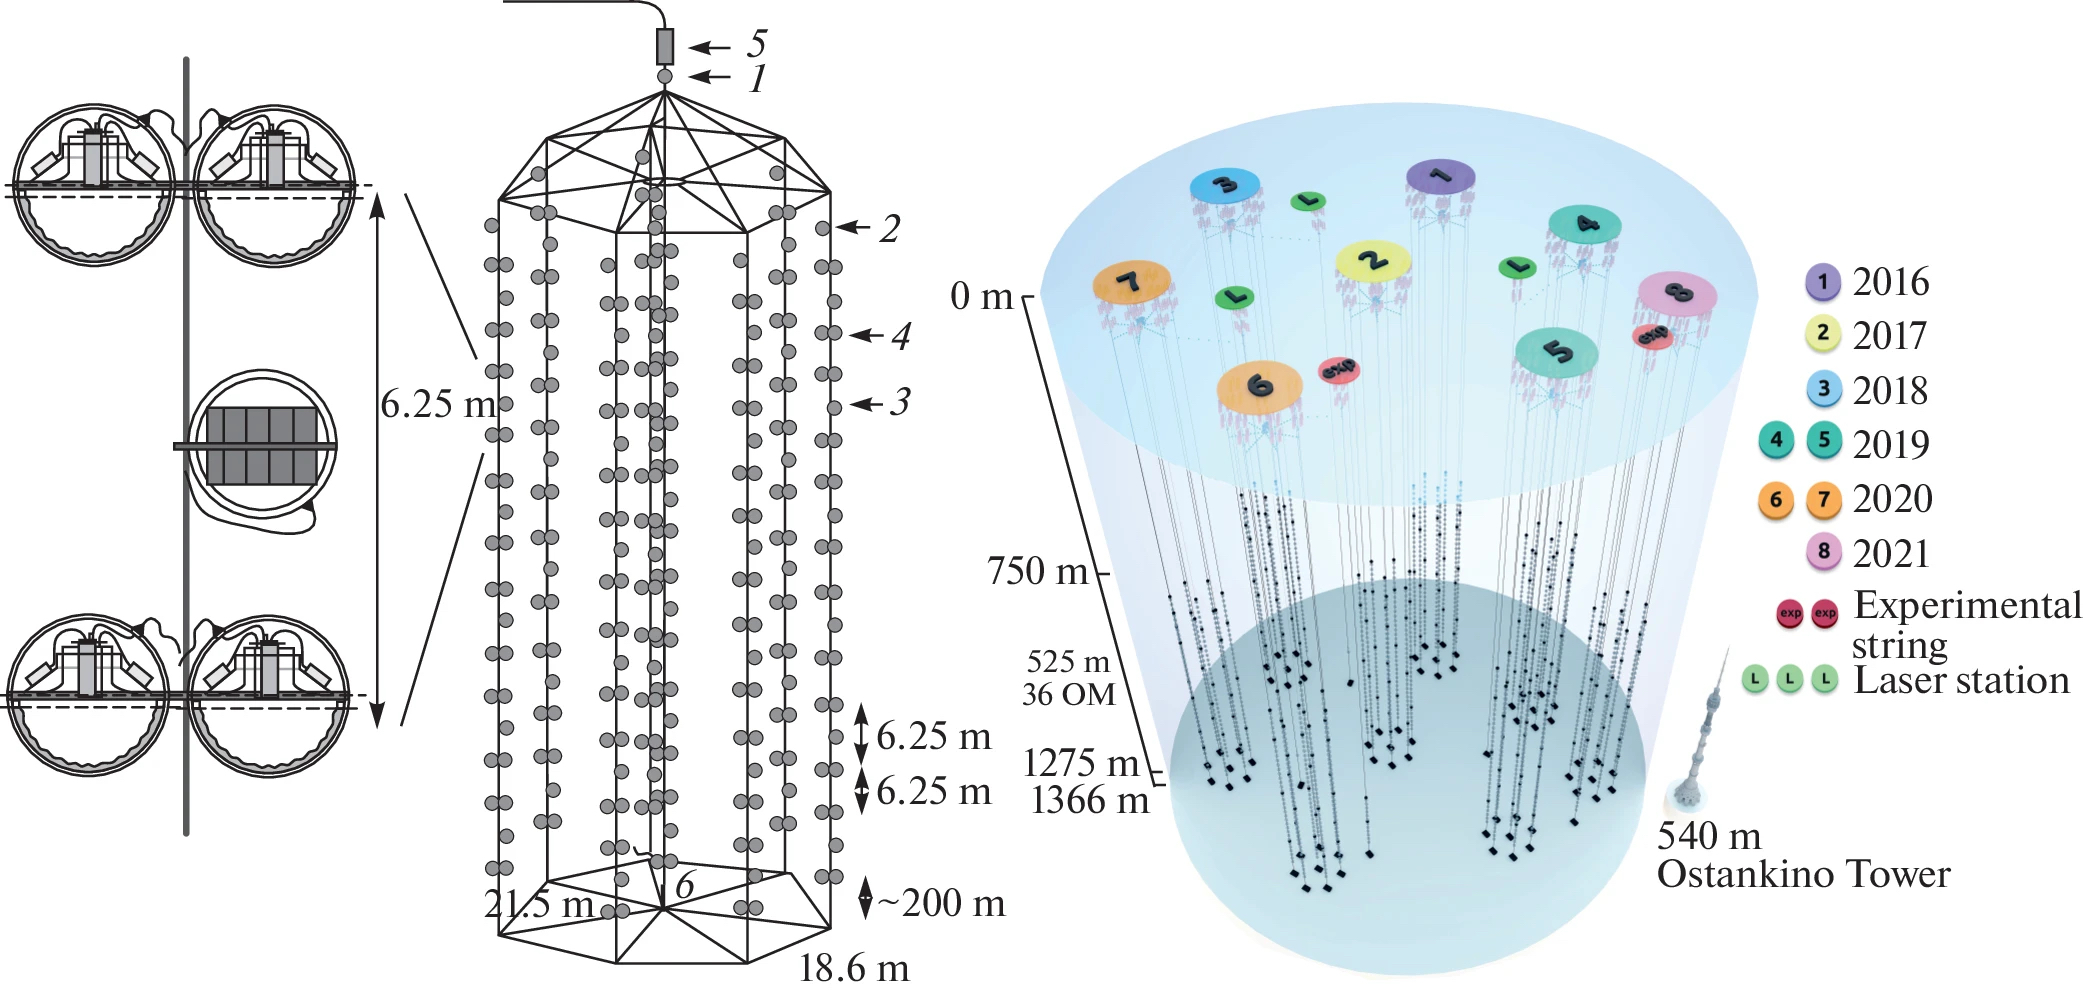
\includegraphics[width=0.9\linewidth]{img/Baikal_scope.jpg}
    \caption{左图,NT-200的探测器阵列示意图。右图,Baikal-GVD目前已经完成的阵列示意图。图片来自\parencite{Baikal_status:2022}}
    \label{fig:Baikal_scope}
\end{figure}

\subsubsection*{KM3NeT}

KM3NeT是Antares的继承项目\cite{KM3Net_letter_of_intent:2016}。KM3NeT中包含两种不同的阵列构成,分别是排布更加稀疏针对高能天体中微子的ARCA,以及排布紧凑用于研究大气中微子振荡的ORCA。
KM3NeT-ARCA规划建设约$1.5\,\mathrm{km^3}$的阵列,目前已经布置了接近10根串列单元。

KM3NeT-ARCA中串列单元之间的平均间距为$90\,\mathrm{m}$,每一根串列单元包含18个mDOM,其间距为$36\,\mathrm{m}$。每一个阵列包含115根串列单元,形成一个半径为$500\,\mathrm{m}$,高度为$612\,\mathrm{m}$的圆柱形探测器阵列。
值得一提的是,KM3NeT中采用了一种独特的滚轮包装方式,可以将一根串列单元打包在一个大型滚球内,实现快速的布放\cite{KM3NeT_deployment:2020}。

\subsubsection*{P-ONE}

P-ONE(Pacific Ocean Neutrino Experiment)是一个正在计划设计中的,位于加拿大西海岸的中微子望远镜实验\cite{P-ONE:2020, P-ONE_ICRC:2021},它的阵列设计如图\ref{fig:P-One_array}中所示。
在目前的设计中,P-ONE类似于Baikal-GVD,由多个区块构成。P-ONE总共包含7个区块,每隔区块包含10根串列单元,每隔串列单元上挂在有20个光学探测模块。其区块和串列单元之间的几何间距如图\ref{fig:P-One_array}中所示。

相比于其他深海中微子望远镜,P-ONE的主要优势是它可以搭载在之前已经建设好的加拿大海底观测网(ONC,Ocean Networks Canada)\cite{P-ONE_ONC:2010},因此其海试实验和装置布放都相对比较容易。

\begin{figure}[!htb]
    \centering
    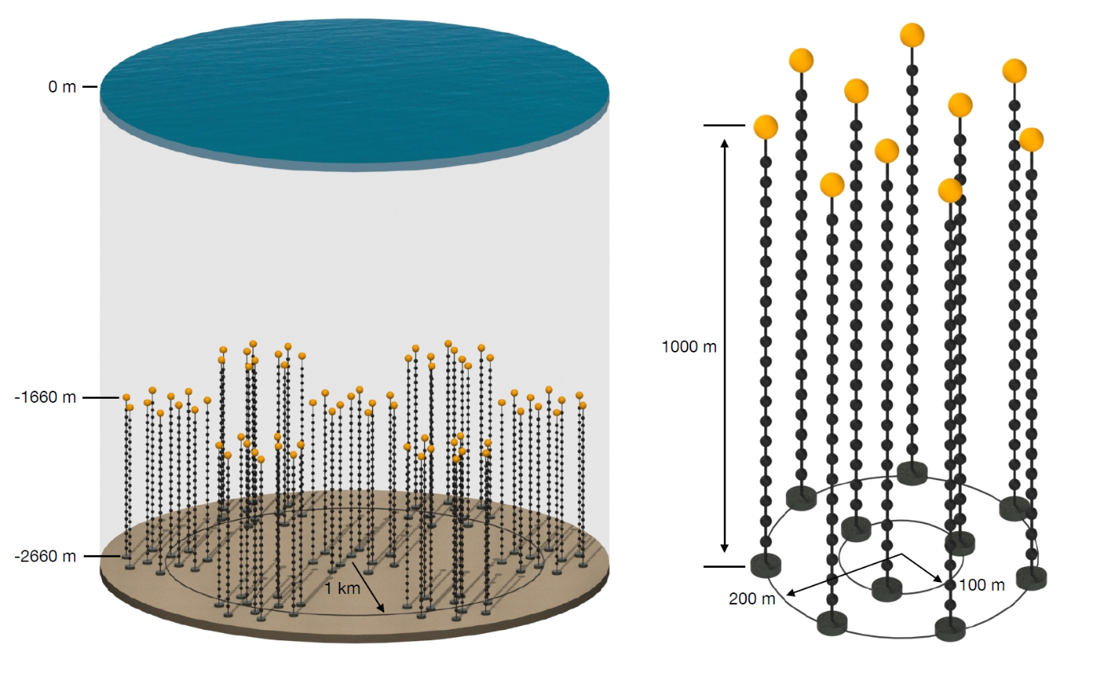
\includegraphics[width=0.8\linewidth]{img/P-One_array.png}
    \caption{P-ONE中微子望远镜阵列的概念设计图。左图:由7个区块组成的整体阵列;右图:单个区块的几何配置。图片来自\parencite{P-ONE_ICRC:2021}}
    \label{fig:P-One_array}
\end{figure}


\subsubsection*{IceCube-Gen2}

IceCube-Gen2是计划中的IceCube的下一代升级版本\cite{IceCube-Gen2_white_paper:2020, IceCube-Gen2_VLVnT:2021}。它计划以几乎相同的DOM数量来覆盖$\sim5\,\mathrm{km^3}$的冰层体积,从而提高探测器的可观测能区。这是由于南极冰川冰中的吸收长度比较长,光子可以在冰内穿行更长的距离。
在目前的设计中,IceCube-Gen2包含120根新的串列单元,串列单元之间的间距为$240\,\mathrm{m}$。每一根串列单元中包含80个DOM,其间距为$15.6\mathrm{m}$,从$1325\,\mathrm{m}$的深度延伸到$2575\,\mathrm{m}$。

除了光学阵列外,IceCube-Gen2还计划在上层冰盖上布置范围更广的射电观测阵列,它们可以用于监测超高能中微子事件中粒子簇射产生的射电信号\cite{IceCube-Gen2_radio:2021}。


\section{海铃中微子望远镜}
\label{sec:TRIDENT_array}

“海铃计划”旨在中国南海建设一座新一代的深海切伦科夫中微子望远镜——海铃中微子望远镜(以下简称为“海铃”),其英文名为TRIDENT(The tRoplcal DEep-sea Neutrino Telescope),其艺术图如\ref{fig:TRIDENT_array}所示。
海铃的地址位于永兴岛东北部的一片深海平原上,其水深约为$3400\,\mathrm{m}$,有关望远镜的选址调查可以参考\ref{chap:pathfinder}。

\begin{figure}[!htb]%
    \centering
    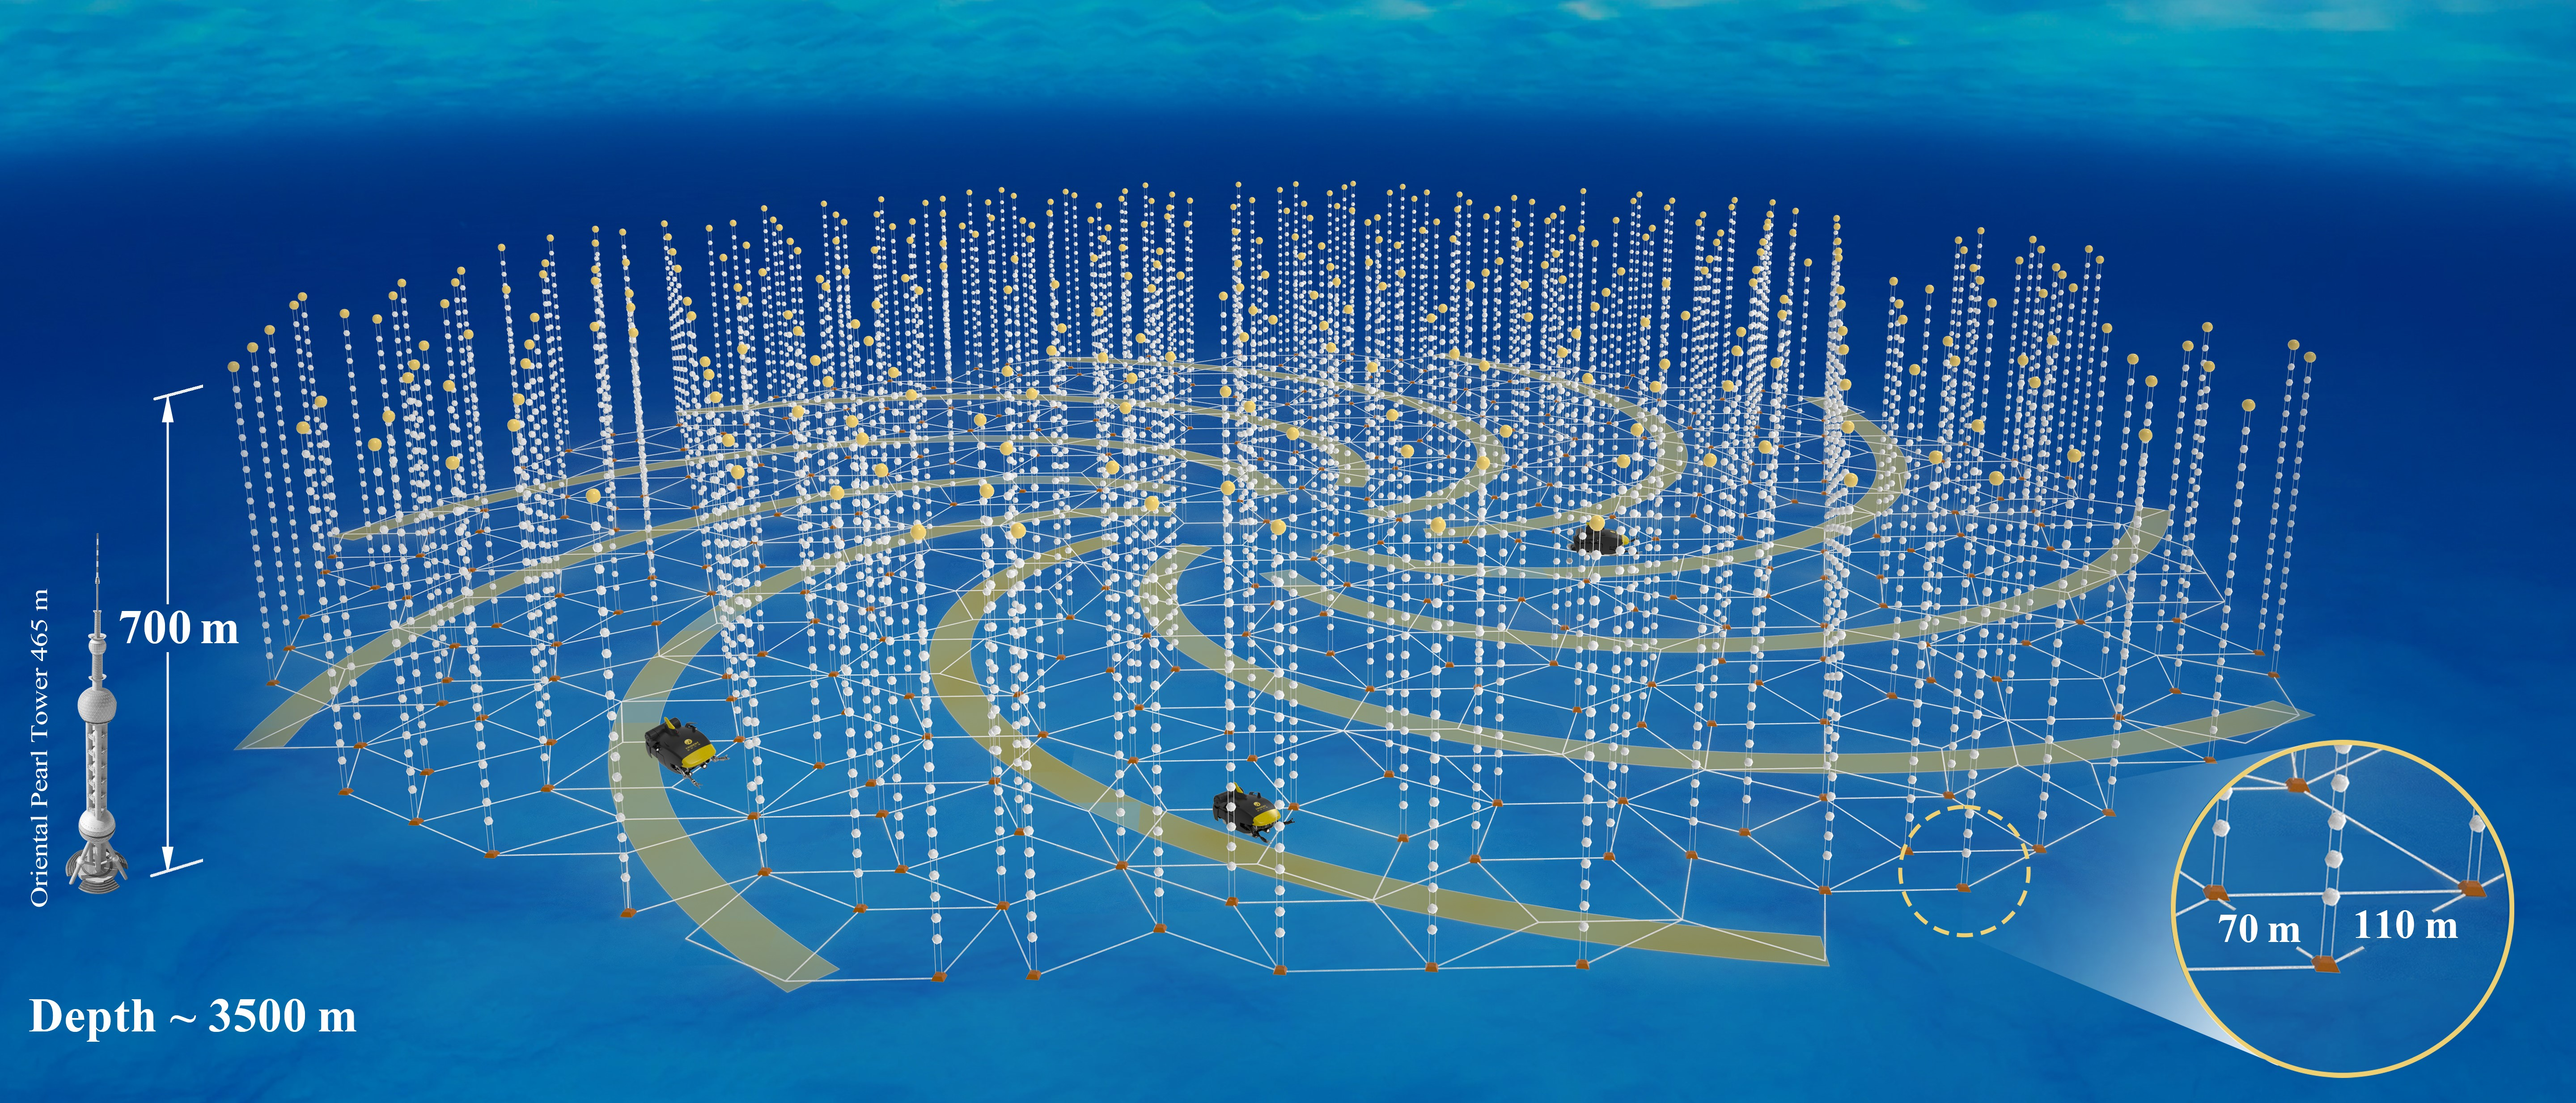
\includegraphics[width=0.95\textwidth]{img/TRIDENT_array.jpeg}
    \caption{海铃的艺术想象图。}
    \label{fig:TRIDENT_array}
\end{figure}

在目前的设计中,海铃采用了彭罗斯镶嵌的结构,其阵列结构如图\ref{fig:geo-layout}所示,图中的每一个黑点表示一根串列单元,图中总共916根串列单元。
这916根串列单元组成了一个半径约$2\,\mathrm{km}$的圆,其覆盖面积约$12\,\mathrm{km^2}$。
串列单元从海底(约3400米深)处延伸至水下2700米,其上分布有20个hDOM,它们之间的垂直间隔为30米,串列单元的高度约$0.7\mathrm{km}$。
海铃的光学探测器阵列的监控体积达到了$7.5\,\mathrm{km^3}$,是目前规划中的最大的新一代中微子望远镜。

在阵列中,我们考虑实际施工布放时的海洋工程要求,在阵列中间留下了一些空隙过道,如图\ref{fig:geo-layout}中虚线所示,我们称之为ROV(Remote Operated Vehicle)过道。这些过道可以将探测器进行适当的分块,防止阵列排布过于紧密导致施工和后期维修困难,方便水下ROV机器人的运作。
为了避免缪子径迹型事件沿着直线直接通过过道穿过阵列而不触发阵列中的hDOM,ROV过道采取了螺旋线型的设计而非简单的直线设计。
需要注意的是目前这些ROV过道对阵列的影响尚未被考虑在模拟研究中,我们在阵列模拟中还是采用了无ROV过道的理想阵列排布,即总探测单元数量为完整的1211根,而非916根。

在阵列布局中,我们同样放置了一些海底次级接驳盒的布置点位,如图\ref{fig:geo-layout}中红色三角形所示。在目前设计的布局中,每一个次级接驳盒可以为附近的20根探测单元提供电力和数据传输的服务,但实际每个次级接驳盒可以供给的探测单元数量由主接驳盒到次级接驳盒的数据传输带宽和供电功率上限决定。

\begin{figure}[!htb]%
    \centering
    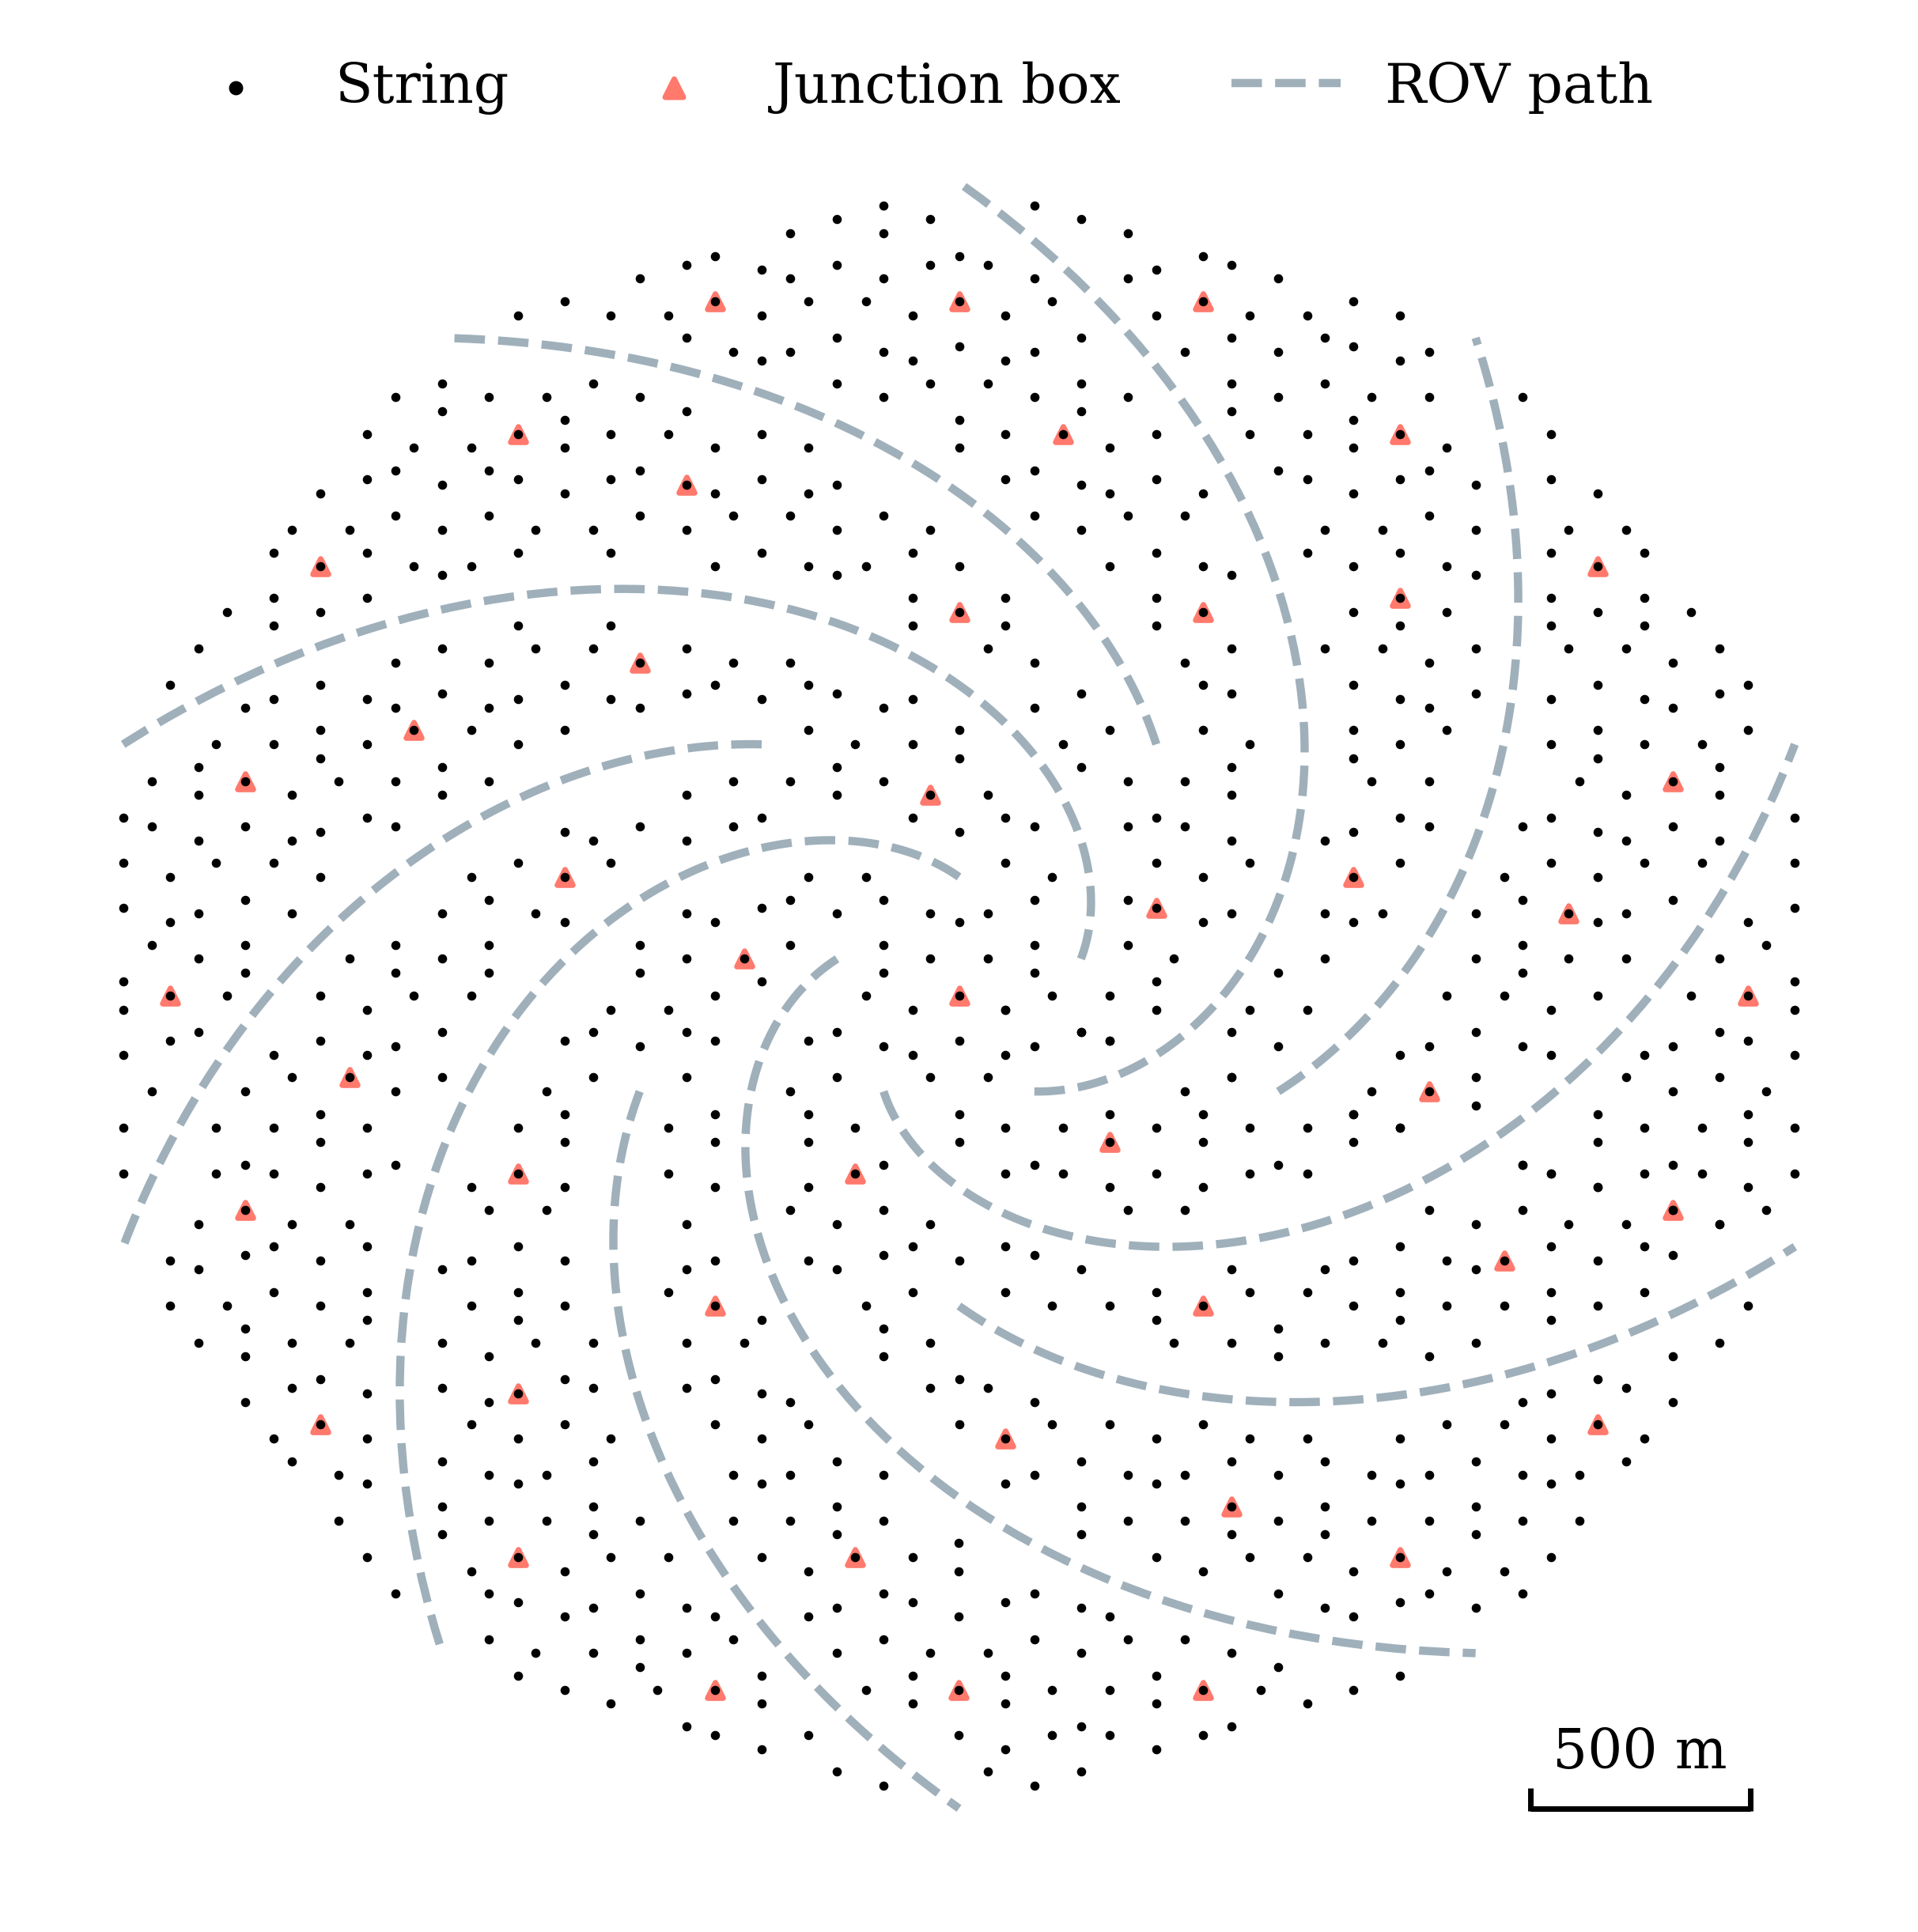
\includegraphics[width=0.85\textwidth]{img/penrose_tiling.png}
    \caption{海铃阵列的集合分布图,其中黑点表示串列单元,红色三角形表示次级接驳盒的位置,蓝色虚线表示ROV过道。}
    \label{fig:geo-layout}
\end{figure}

海铃的主要科学目标是从IceCube观测到的各向同性的弥散高能中微子流寻找产生它们的天体源。海铃庞大的探测器体积为中微子的事例率提供了保障,其优秀的角分辨率可以提高搜寻的灵敏度,有关海铃寻找中微子天体源的性能研究可以参考\ref{chap:telescope_performance}。
其次,海铃还能够研究天体物理尺度基线下的中微子振荡物理。为了实现这个科学目标,对不同中微子味道的分辨能力至关重要。
除了物理研究以外,海铃还是一个多学科研究平台,依托海铃搭建的海底光电缆网络可以布置地球物理和海洋生物研究的探测器。

